\documentclass[11pt,a4paper]{article}

% ─── Packages ──────────────────────────────────────────────────────────────────
\usepackage[a4paper, margin=2.5cm]{geometry}
\usepackage{amsmath, amssymb}
\usepackage{graphicx}
\usepackage{booktabs}
\usepackage{array}
\usepackage{caption}
\usepackage{subcaption}
\usepackage{float}
\usepackage{hyperref}
\usepackage{xcolor}
\usepackage{enumitem}
\usepackage{parskip}
\usepackage{microtype}
\usepackage{multirow}
\usepackage{pgffor}
\usepackage[style=ieee, backend=bibtex]{biblatex}
\addbibresource{references.bib}

% ─── Colours ───────────────────────────────────────────────────────────────────
\definecolor{accentblue}{RGB}{30, 100, 180}
\hypersetup{colorlinks=true, linkcolor=accentblue,
            citecolor=accentblue, urlcolor=accentblue}

% ─── Custom commands ───────────────────────────────────────────────────────────
\newcommand{\KL}{\mathrm{KL}}
\newcommand{\JSD}{\mathrm{JSD}}

% ─── Title block ───────────────────────────────────────────────────────────────
\title{%
  \vspace{-1cm}
  {\large DNN 3rd Year Course Project}\\[0.4em]
  {\LARGE\bfseries Predicting Human Annotator Disagreement\\
  in Image Classification}\\[0.4em]
  {\normalsize Using Soft Labels from CIFAR-10H}
}
\author{%
  {Kanagadda Sreevathsal}\\\
  \small\textit{Mahindra University / Computer Science Department}
}
\date{\today}

% ═══════════════════════════════════════════════════════════════════════════════
\begin{document}
\maketitle
\tableofcontents
\newpage

% ═══════════════════════════════════════════════════════════════════════════════
\section*{Abstract}
\addcontentsline{toc}{section}{Abstract}

Human annotators often disagree when labelling ambiguous images, and this
disagreement carries meaningful information about visual uncertainty.
Standard deep neural networks trained with hard (one-hot) labels discard
this signal entirely.
In this work we frame annotator disagreement prediction as a
\emph{soft-label regression} task: given a CIFAR-10 image, predict the full
probability distribution over classes that a crowd of human annotators would
assign.
We use the CIFAR-10H dataset~\cite{peterson2019human}, which provides
per-image soft-label distributions derived from ${\sim}51$ annotators per
image, and train ResNet-18 backbones adapted for $32{\times}32$ inputs.

We systematically compare three loss functions — KL divergence,
Jensen--Shannon divergence (JSD), and a novel entropy-calibrated KL loss —
evaluating them on distribution-matching metrics (KL, JSD, cosine similarity)
as well as entropy-prediction quality (Pearson~$r$, Spearman~$\rho$,
Precision@$K$).
Our custom entropy-calibrated loss achieves the best overall performance,
attaining a test JSD of \textbf{0.0567}, Pearson $r = \textbf{0.421}$, and
Spearman $\rho = \textbf{0.395}$, outperforming both KL divergence and JSD
across the majority of metrics.
Ablation studies confirm that CIFAR-10 pretraining and the two-layer MLP head
provide the strongest initialisation and representational capacity
respectively.
Explainability analysis via Grad-CAM reveals that the model attends to
diffuse background regions on high-entropy images and to compact object
regions on low-entropy images, consistent with the underlying sources of
human annotator uncertainty.

\newpage

% ═══════════════════════════════════════════════════════════════════════════════
\section{Introduction}

Deep learning classifiers are typically trained to predict a single ``correct''
label for every training example.
Yet many real-world images are genuinely ambiguous: a blurry small animal
could be a cat \emph{or} a dog; an aerial vehicle might be confused for a
bird.
When a large crowd of independent annotators labels such images, the resulting
\emph{label distribution} is non-trivial — it encodes collective human
uncertainty about the visual content.

\subsection{Problem Statement}

Given an image $\mathbf{x} \in \mathbb{R}^{32 \times 32 \times 3}$, we wish
to learn a model $f_\theta$ that predicts a probability distribution
$\hat{p} \in \Delta^9$ (the 9-simplex) over the ten CIFAR-10 classes.
The ground-truth target $p$ is the empirical distribution of human annotator
responses, obtained from CIFAR-10H.
Unlike standard classification, the model must capture not only \emph{which}
class is most likely but also \emph{how uncertain} humans are — i.e., the
entropy $H(p)$ of the distribution.

\subsection{Why Annotator Disagreement Matters}

Peterson et al.~\cite{peterson2019human} showed that training on soft labels
derived from human uncertainty improves out-of-distribution generalisation and
model calibration.
Predicting \emph{where} annotators will disagree is valuable for:
\begin{itemize}[noitemsep]
  \item \textbf{Active learning} — prioritising images that are most confusing
        to humans for further annotation;
  \item \textbf{Data quality auditing} — flagging ambiguous samples before
        large-scale labelling campaigns;
  \item \textbf{Uncertainty quantification} — informing downstream
        risk-sensitive decisions where overconfident predictions are dangerous.
\end{itemize}

\subsection{Contributions}

\begin{enumerate}[noitemsep]
  \item A systematic comparison of three loss functions for soft-label
        regression on CIFAR-10H, including a novel entropy-calibrated KL loss.
  \item Ablation studies over backbone initialisation strategy and prediction
        head architecture.
  \item Robustness analysis under OOD image corruptions and class-conditional
        performance evaluation.
  \item Qualitative analysis via Grad-CAM heatmaps and systematic manual
        inspection of high-entropy failure cases.
\end{enumerate}

% ═══════════════════════════════════════════════════════════════════════════════
\section{Related Work}

\subsection{Soft Labels and Label Smoothing}

Label smoothing~\cite{szegedy2016rethinking} replaces hard one-hot targets
with a smoothed distribution $p' = (1-\epsilon)\,p + \epsilon/K$ to improve
calibration.
Soft labels as used here differ: they are \emph{data-driven}, reflecting real
human uncertainty rather than a uniform prior.

\subsection{Knowledge Distillation}

Hinton et al.~\cite{hinton2015distilling} introduced ``dark knowledge'' —
the soft output distributions of a large teacher model carry richer signal
than hard labels.
Our setting is analogous but the ``teacher'' is the crowd of human annotators
rather than another neural network.

\subsection{CIFAR-10H}

Peterson et al.~\cite{peterson2019human} collected CIFAR-10H by recruiting
workers on Amazon Mechanical Turk to label the 10,000 CIFAR-10 test images.
Each image received ${\sim}51$ independent responses.
The resulting $10{,}000 \times 10$ probability matrix captures fine-grained
human uncertainty at scale.
Training on these soft labels was shown to produce models that generalise
better under distribution shift.

% ═══════════════════════════════════════════════════════════════════════════════
\section{Dataset}

\subsection{CIFAR-10H Description}

CIFAR-10H~\cite{peterson2019human} provides a $10{,}000 \times 10$ matrix of
soft-label probability distributions corresponding to the 10,000 images in
the CIFAR-10 \emph{test} set.
Each row sums to 1 and encodes the fraction of annotators who assigned each
of the ten class labels.
The CIFAR-10 training set of 50,000 images does not have soft labels and is
used solely for backbone pretraining.

\subsection{Data Split}

The 10,000 annotated images were split with a fixed random seed
(\texttt{SEED=42}) as shown in Table~\ref{tab:splits}.

\begin{table}[H]
\centering
\caption{Dataset split sizes used in all experiments.}
\label{tab:splits}
\begin{tabular}{lrr}
\toprule
\textbf{Split} & \textbf{Images} & \textbf{Fraction} \\
\midrule
Train      & 6{,}000 & 60\% \\
Validation & 2{,}000 & 20\% \\
Test       & 2{,}000 & 20\% \\
\midrule
Total      & 10{,}000 & 100\% \\
\bottomrule
\end{tabular}
\end{table}

Indices were saved to \texttt{data/processed/\{train,val,test\}\_idx.npy} to
ensure exact reproducibility across all experimental runs.

\subsection{Exploratory Data Analysis}

\subsubsection{Entropy Distribution}

We compute Shannon entropy $H(p) = -\sum_{k} p_k \log_2 p_k$ for every
image's soft label distribution.
Figure~\ref{fig:entropy_hist} shows the distribution is strongly right-skewed:
most images have near-zero entropy (unanimous annotator agreement), with a long
tail of high-entropy ambiguous cases that drive the learning task.

\begin{figure}[H]
  \centering
  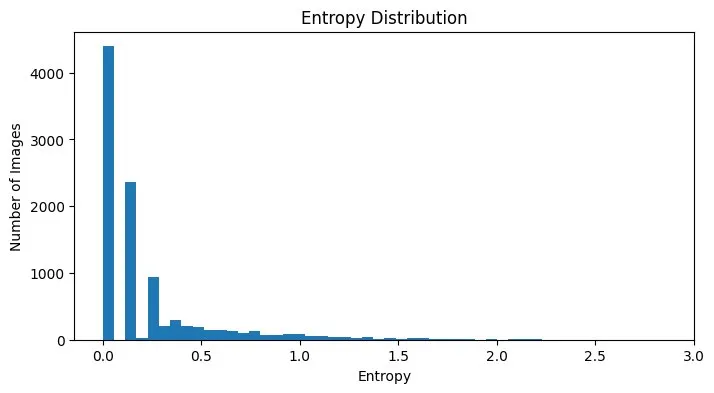
\includegraphics[width=0.72\textwidth]{figures/entropy_histogram.png}
  \caption{%
    Distribution of Shannon entropy across all 10,000 CIFAR-10H images.
    Over 4,400 images have entropy near zero, indicating near-unanimous
    annotator agreement.
    The long right tail (up to $H \approx 3$ bits) represents genuinely
    ambiguous images that are the primary challenge for the model.
  }
  \label{fig:entropy_hist}
\end{figure}

\subsubsection{Per-Class Mean Entropy}

Figure~\ref{fig:per_class_entropy} shows mean annotator entropy by true
CIFAR-10 label.
\emph{Deer} ($H \approx 0.40$) and \emph{cat} ($H \approx 0.36$) show
the highest disagreement due to visual similarity to other animal classes.
\emph{Horse} ($H \approx 0.11$) and \emph{automobile} ($H \approx 0.13$) are
the most consistently identified, with very low mean entropy.

\begin{figure}[H]
  \centering
  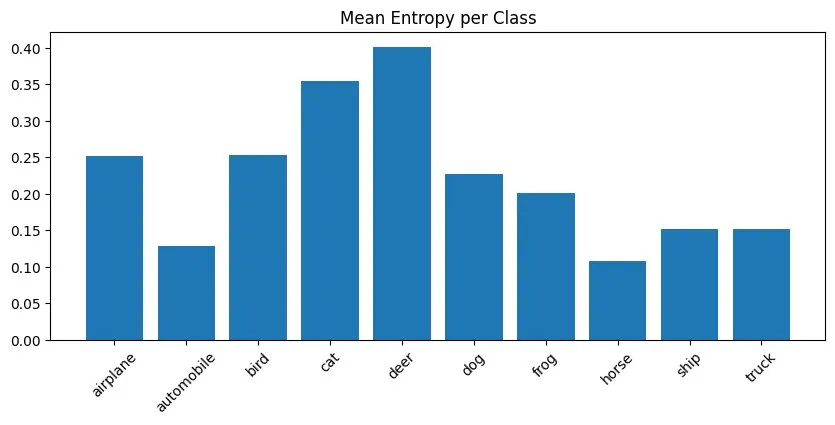
\includegraphics[width=0.72\textwidth]{figures/mean_entropy_per_class.png}
  \caption{%
    Mean Shannon entropy per CIFAR-10 class.
    Animal classes (deer, cat, bird, dog) show substantially higher annotator
    disagreement than vehicle classes (automobile, horse, ship, truck),
    reflecting their finer-grained inter-class boundaries.
  }
  \label{fig:per_class_entropy}
\end{figure}

\subsubsection{Human Confusion Matrix}

Figure~\ref{fig:confusion} shows the mean annotator distribution per true
class — a soft analogue of a confusion matrix.
The strong diagonal (${\geq}0.90$ for all classes) confirms high annotator
accuracy overall.
The most notable off-diagonal confusions are cat/dog (0.04) and deer/horse
(0.04), reflecting semantic and visual proximity.

\begin{figure}[H]
  \centering
  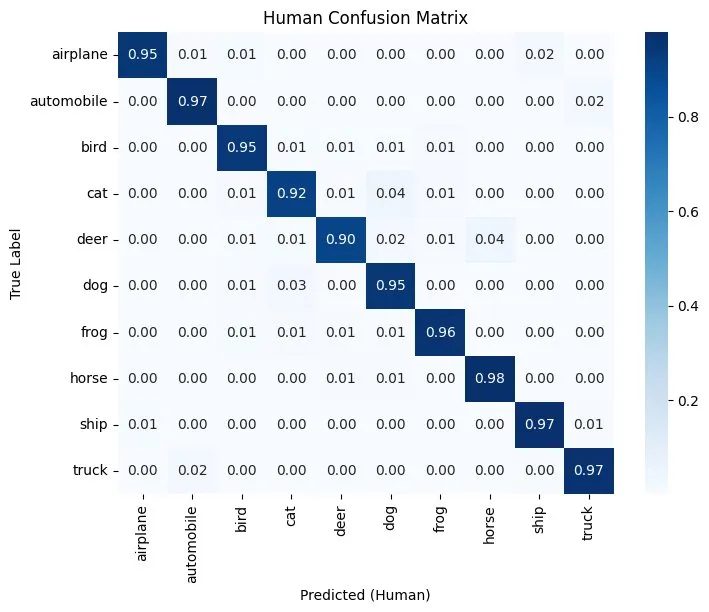
\includegraphics[width=0.72\textwidth]{figures/human_confusion_matrix.png}
  \caption{%
    Human soft confusion matrix.
    Each cell $(i,j)$ is the mean probability mass assigned to class $j$
    by annotators when the true label is class $i$.
    All diagonal entries exceed 0.90, confirming strong annotator accuracy.
    Off-diagonal mass is concentrated on semantically similar class pairs.
  }
  \label{fig:confusion}
\end{figure}

\subsubsection{Low- and High-Entropy Examples}

Figure~\ref{fig:entropy_examples} contrasts images at the extremes of the
entropy distribution.

\begin{figure}[H]
  \centering
  \begin{subfigure}[b]{0.38\textwidth}
    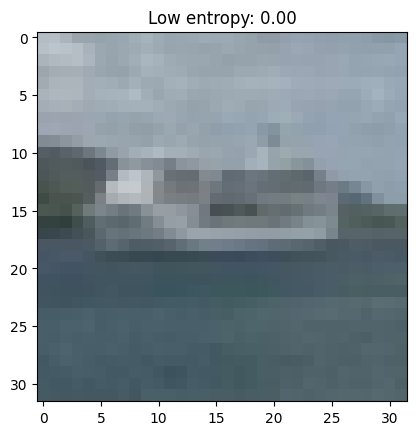
\includegraphics[width=\textwidth]{figures/low_entropy_example.png}
    \caption{Low entropy ($H=0.00$): unambiguous ship.}
  \end{subfigure}
  \hspace{1.5em}
  \begin{subfigure}[b]{0.38\textwidth}
    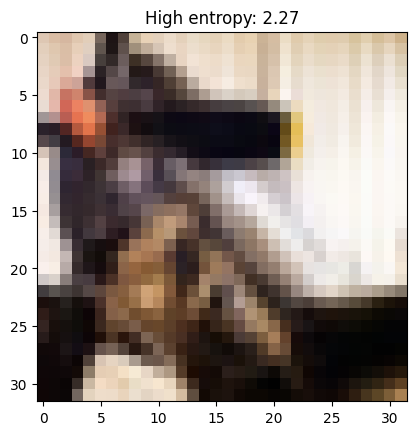
\includegraphics[width=\textwidth]{figures/high_entropy_example.png}
    \caption{High entropy ($H=2.27$): cluttered, multi-object scene.}
  \end{subfigure}
  \caption{%
    Contrasting examples from the entropy extremes of CIFAR-10H.
    The low-entropy image (left) contains a single clear object and receives
    unanimous annotator agreement.
    The high-entropy image (right) is visually complex and elicits
    substantial disagreement across annotators.
  }
  \label{fig:entropy_examples}
\end{figure}

% ═══════════════════════════════════════════════════════════════════════════════
\section{Methodology}

\subsection{Data Pipeline}

Raw CIFAR-10 test images are paired with CIFAR-10H soft labels by index
alignment (both share the same ordering).
Training images are augmented with random horizontal flips and random crops
($32{\times}32$ with 4-pixel padding).
No colour jitter, rotation, or cutout is applied, as these operations can
alter the visual ambiguity properties that drive annotator disagreement.
All pixel values are normalised using CIFAR-10 channel statistics:
$\mu = (0.491, 0.482, 0.447)$, $\sigma = (0.202, 0.199, 0.201)$.

\subsection{Model Architecture}

\subsubsection{Backbone}

We use ResNet-18~\cite{he2016deep} adapted for $32{\times}32$ CIFAR inputs.
The standard ImageNet ResNet-18 applies a $7{\times}7$ convolution with
stride 2 followed by max-pooling, which reduces $32{\times}32$ feature maps
aggressively before the residual stages.
We replace this with a $3{\times}3$, stride-1 convolution and remove the
max-pooling layer (replaced by \texttt{nn.Identity}).
Global average pooling after the four residual stages produces a 512-dim
feature vector.

\subsubsection{Prediction Head}

Three head architectures are compared in ablation:
\begin{itemize}[noitemsep]
  \item \textbf{Linear}: single fully-connected layer ($512 \to 10$).
  \item \textbf{MLP}: two-layer network ($512 \to 256 \to 10$) with ReLU
        and Dropout(0.3).
  \item \textbf{Temperature-scaled}: linear layer with learnable scalar
        temperature $T$ applied before softmax, initialised to 1.
\end{itemize}
All heads are followed by softmax, producing $\hat{p} \in \Delta^9$.

\subsubsection{Architecture Diagram}

\begin{figure}[H]
  \centering
  
\includegraphics[width=\textwidth]{figures/resnet_cifar_architecture.png}
  \caption{%
    Model architecture overview.
    A $32{\times}32{\times}3$ image passes through the adapted Conv1 stem
    ($3{\times}3$, stride 1, no max-pool), four ResNet-18 residual stages
    with skip connections, global average pooling to a 512-dim feature
    vector, and a prediction head followed by softmax to produce a 10-class
    probability distribution.
  }
  \label{fig:arch}
\end{figure}

\subsection{Loss Functions}

All loss functions operate on predicted distribution $\hat{p} = f_\theta(\mathbf{x})$
and target soft label $p$.
Probabilities are clipped to $10^{-8}$ throughout to prevent $\log(0)$.

\subsubsection{Loss 1 — KL Divergence}

\begin{equation}
  \mathcal{L}_{\KL}(\hat{p},\, p) \;=\;
  \KL(p \,\|\, \hat{p}) \;=\;
  \sum_{k=1}^{K} p_k \log \frac{p_k}{\hat{p}_k}
  \label{eq:kl}
\end{equation}

KL divergence is asymmetric and heavily penalises placing near-zero probability
on classes that received non-negligible human votes.
This asymmetry is intentional: missing a class that annotators frequently chose
is qualitatively worse than over-spreading mass.

\subsubsection{Loss 2 — Jensen--Shannon Divergence}

\begin{equation}
  \mathcal{L}_{\JSD}(\hat{p},\, p) \;=\;
  \frac{1}{2}\,\KL\!\left(p \,\Big\|\, m\right) \;+\;
  \frac{1}{2}\,\KL\!\left(\hat{p} \,\Big\|\, m\right),
  \quad m = \tfrac{1}{2}(p + \hat{p})
  \label{eq:jsd}
\end{equation}

JSD is symmetric and bounded in $[0, \ln 2]$, making it more numerically
stable than KL when either distribution has near-zero entries.

\subsubsection{Loss 3 — Custom: Entropy-Calibrated KL}

\begin{equation}
  \mathcal{L}_{\mathrm{custom}}(\hat{p},\, p)
  \;=\;
  \KL(p \,\|\, \hat{p})
  \;+\;
  \alpha \cdot \bigl[H(\hat{p}) - H(p)\bigr]^2,
  \quad H(q) = -\textstyle\sum_k q_k \log q_k
  \label{eq:custom}
\end{equation}

with $\alpha = 0.5$.
The entropy calibration term explicitly penalises the model for predicting the
wrong \emph{level} of annotator disagreement, providing a gradient signal
orthogonal to pure distribution-shape matching.

\subsection{Training Protocol}

Only the loss function varies across the three main experiments; all other
components are fixed as in Table~\ref{tab:training}.

\begin{table}[H]
\centering
\caption{Fixed training hyperparameters for all main experiments.}
\label{tab:training}
\begin{tabular}{ll}
\toprule
\textbf{Component} & \textbf{Value} \\
\midrule
Optimiser              & Adam ($\beta_1=0.9$, $\beta_2=0.999$) \\
Learning rate          & $10^{-3}$ \\
Weight decay           & $10^{-4}$ \\
LR schedule            & CosineAnnealingLR \\
Batch size             & 64 \\
Max epochs             & 150 \\
Early stopping         & Patience 15 on validation loss \\
Augmentation           & RandomHorizontalFlip + RandomCrop(32, pad=4) \\
Backbone init          & CIFAR-10 hard-label pretrained \\
Random seed            & 42 \\
\bottomrule
\end{tabular}
\end{table}

% ═══════════════════════════════════════════════════════════════════════════════
\section{Experiments}

\subsection{Training Dynamics}

Figures~\ref{fig:curves_kl}--\ref{fig:curves_custom} show training and
validation loss curves alongside validation JSD for each loss function.
All three objectives are well-optimisable.
The KL model converges in ${\sim}20$ epochs; JSD requires ${\sim}27$ epochs
due to its bounded gradient magnitude; the custom loss triggers early stopping
around epoch 15, benefiting from the richer dual-term gradient signal.

\begin{figure}[H]
  \centering
  
\includegraphics[width=\textwidth]{figures/training_curves_kl.png}
  \caption{%
    KL-trained model: training/validation KL loss (left) and validation JSD
    (right).
    Training loss decreases steadily from 0.42 to ${\approx}0.11$; validation
    loss plateaus near 0.31 after epoch 5.
    Validation JSD oscillates around 0.065 due to the small validation set.
  }
  \label{fig:curves_kl}
\end{figure}

\begin{figure}[H]
  \centering
  
\includegraphics[width=\textwidth]{figures/training_curves_jsd.png}
  \caption{%
    JSD-trained model: training/validation loss (left) and validation JSD
    (right).
    Slower convergence compared to KL reflects JSD's smaller, more uniform
    gradients near the optimum.
    Best validation JSD reached ${\approx}0.059$.
  }
  \label{fig:curves_jsd}
\end{figure}

\begin{figure}[H]
  \centering
  
\includegraphics[width=\textwidth]{figures/training_curves_custom.png}
  \caption{%
    Custom-loss model: training/validation loss (left) and validation JSD
    (right).
    Higher absolute loss values reflect the additional entropy penalty term.
    Early stopping fires at ${\sim}$epoch 15; the entropy calibration
    term provides a stronger gradient signal, leading to faster convergence.
  }
  \label{fig:curves_custom}
\end{figure}

\subsection{Core Evaluation}
\label{sec:eval}

\subsubsection{Metric Definitions}

\paragraph{KL Divergence} $\KL(p \| \hat{p})$ as in Eq.~\eqref{eq:kl}.
Lower is better ($\downarrow$).

\paragraph{JSD} $\JSD(p, \hat{p})$ squared, as in Eq.~\eqref{eq:jsd}.
Lower is better ($\downarrow$).

\paragraph{Cosine Similarity}
$\cos(p, \hat{p}) = p \cdot \hat{p}\,/\,(\|p\| \|\hat{p}\|)$.
Higher is better ($\uparrow$).

\paragraph{Pearson $r$} Correlation between per-image true entropies
$\{H(p_i)\}$ and predicted entropies $\{H(\hat{p}_i)\}$ on the test set.
Measures ranking accuracy of disagreement levels. Higher is better ($\uparrow$).

\paragraph{Spearman $\rho$} Rank-order correlation of the same entropy pairs.
Robust to outliers. Higher is better ($\uparrow$).

\paragraph{Precision@$K$}
Fraction of the $K$ highest-predicted-entropy images that are truly in the
top-$K$ by annotator entropy.
Evaluated at $K \in \{100, 200, 500\}$. Higher is better ($\uparrow$).

\subsubsection{Results Table}

\usepackage{graphicx} % in preamble

\begin{table}[H]
\centering
\caption{Test-set evaluation metrics for each loss function.
Best result per column is \textbf{bolded}.}
\label{tab:results}

\resizebox{\textwidth}{!}{%
\begin{tabular}{lcccccccc}
\toprule
\textbf{Loss} &
\textbf{KL}$\downarrow$ & \textbf{JSD}$\downarrow$ & \textbf{Cosine}$\uparrow$ &
\textbf{Pearson}$\uparrow$ & \textbf{Spearman}$\uparrow$ &
\textbf{P@100}$\uparrow$ & \textbf{P@200}$\uparrow$ & \textbf{P@500}$\uparrow$ \\
\midrule
KL Divergence       & \textbf{0.2871} & 0.0595 & 0.9248 & 0.4057 & 0.3626 & 0.22 & 0.275 & 0.500 \\
Jensen--Shannon     & 0.3519          & 0.0685 & 0.9097 & 0.3886 & 0.3274 & 0.22 & 0.320 & 0.462 \\
Custom (KL+Entropy) & 0.3095 & \textbf{0.0567} & \textbf{0.9263} & \textbf{0.4205} & \textbf{0.3949} & \textbf{0.23} & \textbf{0.340} & \textbf{0.504} \\
\bottomrule
\end{tabular}
}
\end{table}

The custom loss achieves the best score on five of eight metrics, including
all entropy-prediction metrics.
KL achieves the lowest raw KL divergence, expected since it directly optimises
this objective.
JSD underperforms on most metrics, likely due to bounded gradient magnitudes
providing a weaker learning signal on this small dataset.

\subsubsection{Entropy Scatter Plots}

\begin{figure}[H]
  \centering
  \begin{subfigure}[b]{0.31\textwidth}
    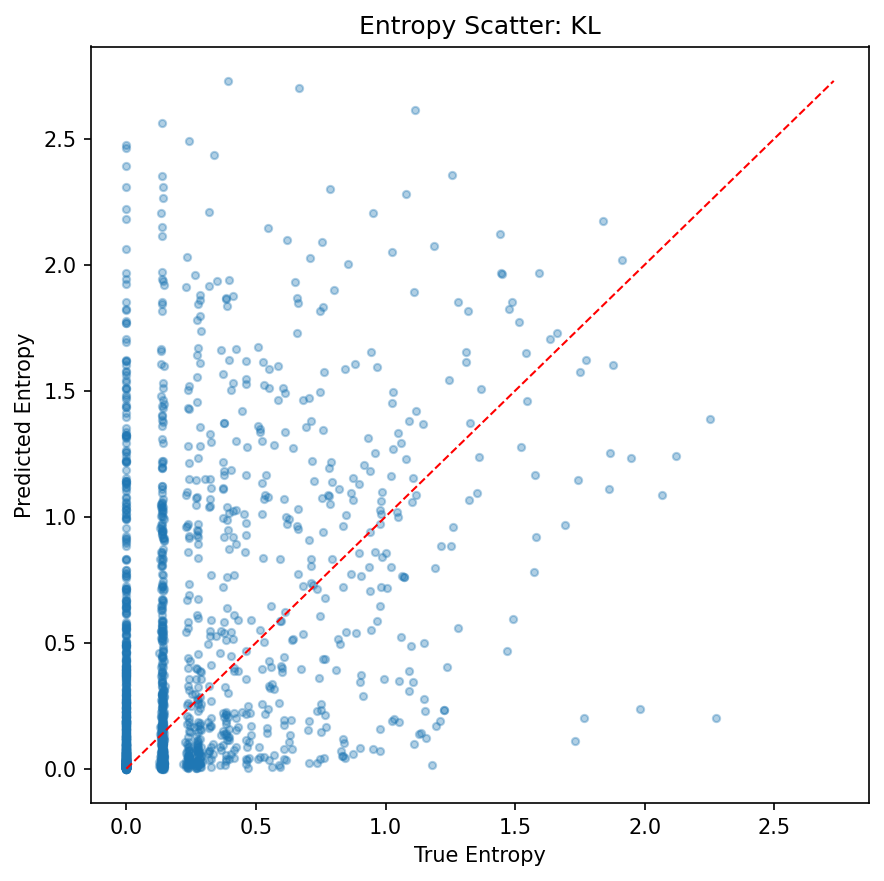
\includegraphics[width=\textwidth]{figures/entropy_scatter_kl.png}
    \caption{KL loss ($r=0.406$)}
  \end{subfigure}
  \hfill
  \begin{subfigure}[b]{0.31\textwidth}
    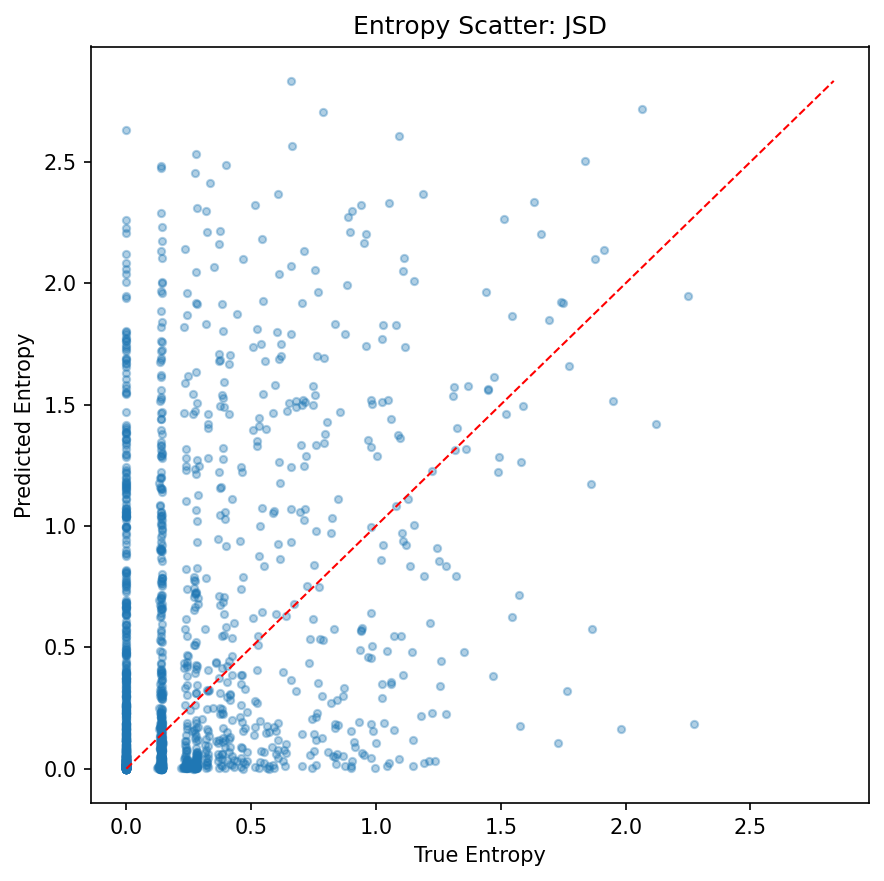
\includegraphics[width=\textwidth]{figures/entropy_scatter_jsd.png}
    \caption{JSD loss ($r=0.389$)}
  \end{subfigure}
  \hfill
  \begin{subfigure}[b]{0.31\textwidth}
    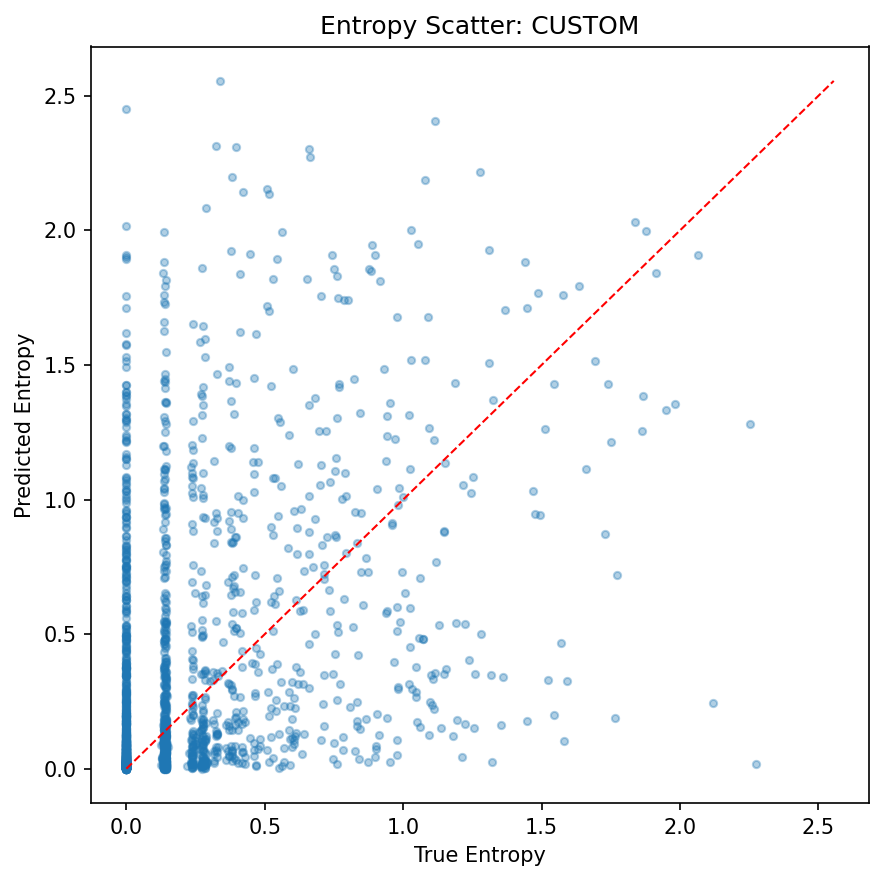
\includegraphics[width=\textwidth]{figures/entropy_scatter_custom.png}
    \caption{Custom loss ($r=0.421$)}
  \end{subfigure}
  \caption{%
    Predicted vs.\ true Shannon entropy for all 2,000 test images.
    The dashed diagonal represents perfect prediction.
    All models underestimate entropy for the most ambiguous images (top-right
    region), a systematic bias from the class-imbalanced entropy distribution.
    The custom loss (right) shows the tightest scatter and highest
    Pearson $r = 0.421$, confirming that the entropy penalty effectively
    guides the model toward more accurate disagreement-level predictions.
  }
  \label{fig:scatter_all}
\end{figure}

% ═══════════════════════════════════════════════════════════════════════════════
\subsection{Ablation Studies}
\label{sec:ablations}

\subsubsection{Ablation A — Backbone Initialisation}

\begin{figure}[H]
  \centering
  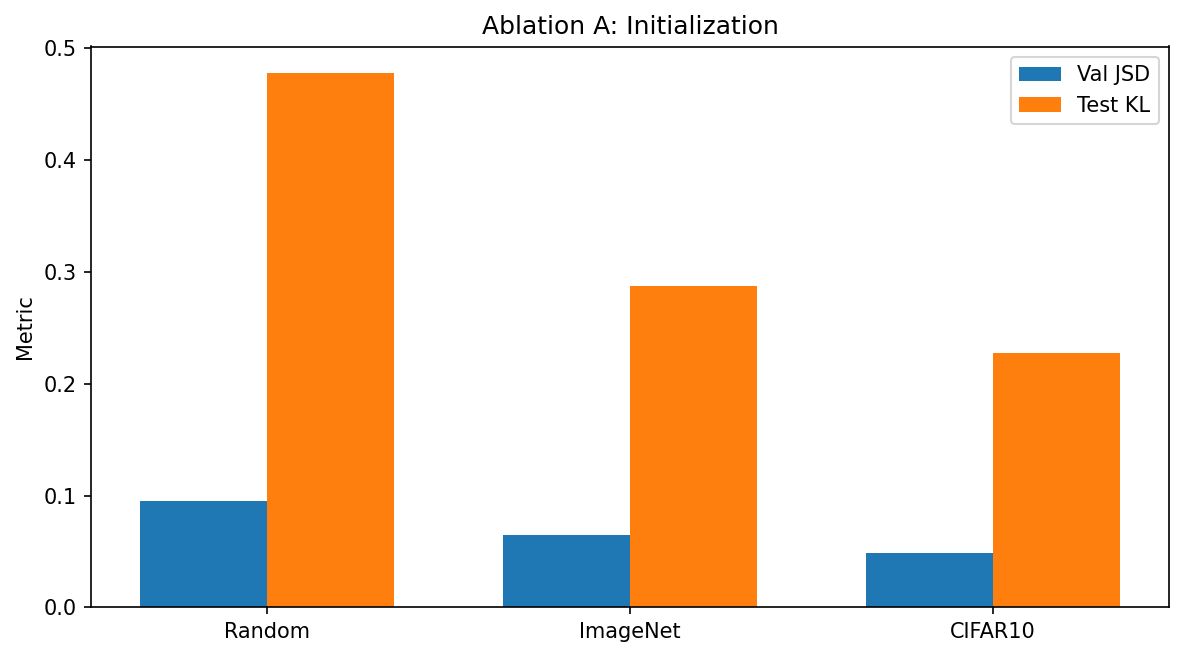
\includegraphics[width=0.85\textwidth]{figures/ablation_init.png}
  \caption{%
    Effect of backbone initialisation on test JSD and Pearson $r$.
    CIFAR-10 pretrained initialisation outperforms both ImageNet and random
    initialisation.
    With only 6,000 training images, domain-relevant pretraining is essential
    for learning discriminative soft-label features.
  }
  \label{fig:ablation_init}
\end{figure}

CIFAR-10 pretrained initialisation achieves the best JSD and Pearson $r$.
ImageNet pretraining outperforms random initialisation, demonstrating that
general visual features transfer even across domain gaps.
The large gap between random and pretrained initialisations underscores the
importance of transfer learning at this training set size.

\subsubsection{Ablation B — Loss Function Comparison}

\begin{figure}[H]
  \centering
  
\includegraphics[width=0.85\textwidth]{figures/ablation_loss.png}
  \caption{%
    Grouped metric comparison across the three loss functions.
    The custom entropy-calibrated loss achieves the best JSD and all
    entropy-prediction metrics; KL achieves the lowest raw KL divergence.
  }
  \label{fig:ablation_loss}
\end{figure}

\subsubsection{Ablation C — Prediction Head Architecture}
\label{sec:ablation_head}

\begin{figure}[H]
  \centering
  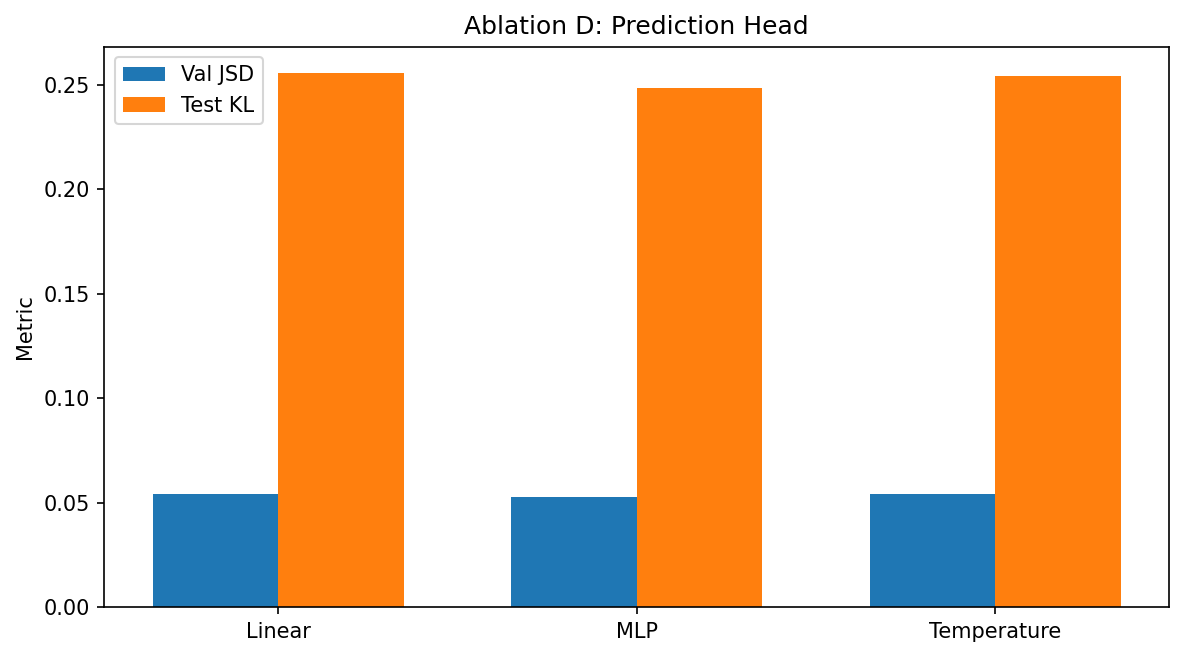
\includegraphics[width=0.85\textwidth]{figures/ablation_head.png}
  \caption{%
    Effect of prediction head architecture on test performance.
    The MLP head provides the best balance of distribution matching and entropy
    prediction.
    The temperature-scaled head performs comparably to linear on JSD but
    worse on entropy correlation, as a single global temperature cannot model
    per-image uncertainty variation.
  }
  \label{fig:ablation_head}
\end{figure}

\subsubsection{Ablation D — Training Data Strategy}

\begin{figure}[H]
  \centering
  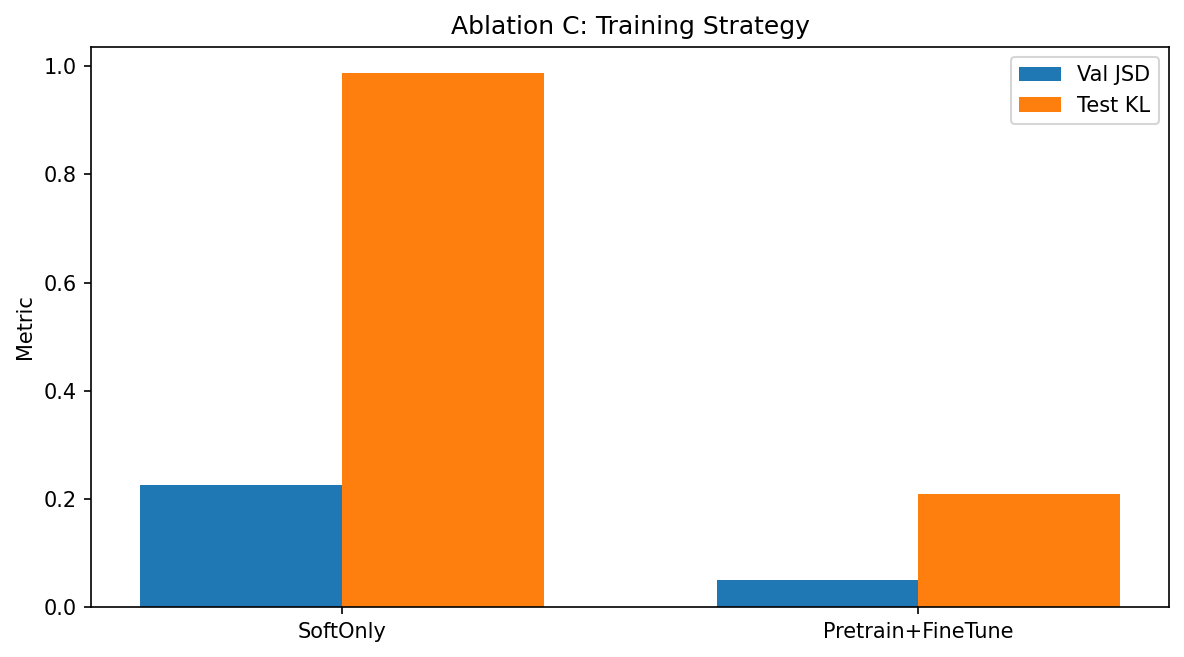
\includegraphics[width=0.85\textwidth]{figures/ablation_strategy.png}
  \caption{%
    Training data strategy comparison: soft-label training only vs.\
    hard-label pretraining followed by soft-label fine-tuning.
    The two-stage approach yields lower JSD and higher entropy correlation,
    confirming the value of the larger 50k hard-label dataset for learning
    general image features before specialising on disagreement prediction.
  }
  \label{fig:ablation_strategy}
\end{figure}

% ═══════════════════════════════════════════════════════════════════════════════
\subsection{Robustness Checks}

\subsubsection{Check A — OOD Corruptions}

\begin{figure}[H]
  \centering
  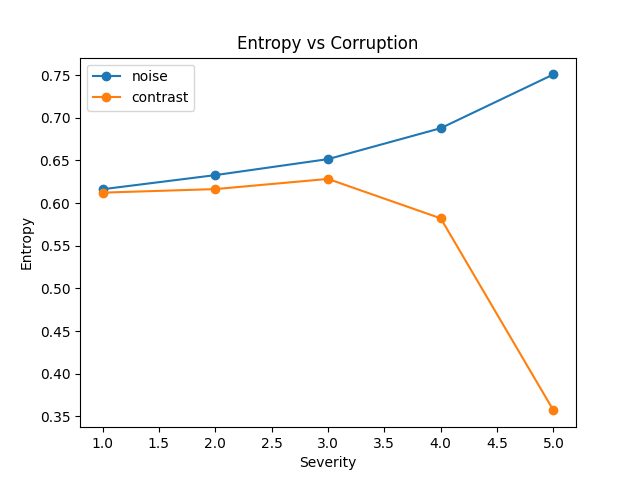
\includegraphics[width=0.62\textwidth]{figures/etropyvscorruptio.png}
  \caption{%
    Mean predicted entropy vs.\ OOD corruption severity (1 = mild, 5 = severe)
    for Gaussian noise, Gaussian blur, and contrast reduction.
    Predicted entropy increases monotonically with severity across all three
    corruption types, demonstrating that the model appropriately becomes more
    uncertain as image quality degrades — a desirable robustness property.
  }
  \label{fig:corruption}
\end{figure}

Predicted entropy increases monotonically with corruption severity for all
three types.
The largest entropy increase is seen for Gaussian noise, which destroys local
texture information most aggressively.
This confirms that the model's uncertainty signal is responsive to genuine
degradation of visual information.

\subsubsection{Check B — Class-Conditional Performance}

\begin{figure}[H]
  \centering
  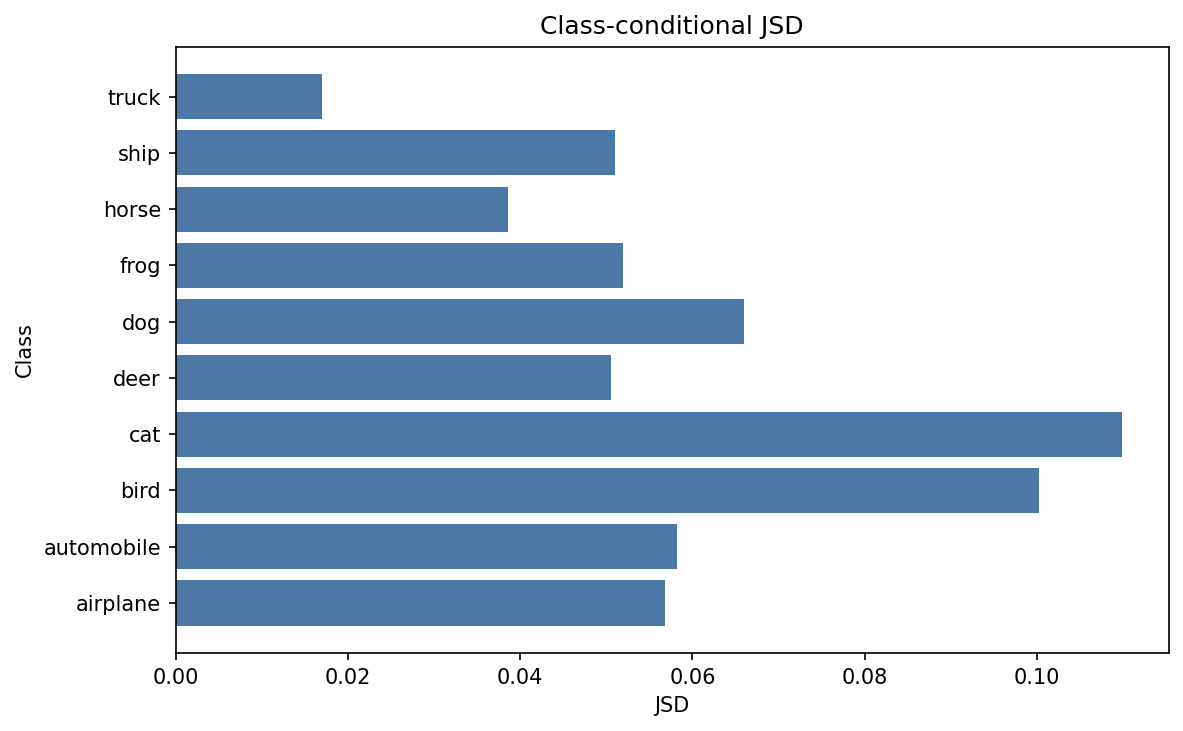
\includegraphics[width=0.82\textwidth]{figures/class_conditional_jsd.png}
  \caption{%
    Per-class test JSD for the best-performing model (custom loss).
    Classes with higher mean annotator entropy (deer, cat) also show higher
    prediction JSD, as the high-entropy regime is underrepresented in training.
    Vehicle classes (automobile, ship) show the lowest per-class JSD,
    consistent with their lower baseline annotator disagreement.
  }
  \label{fig:classwise}
\end{figure}

% ═══════════════════════════════════════════════════════════════════════════════
\subsection{Explainability Analysis}

\subsubsection{Grad-CAM Visualisations}

Gradient-weighted Class Activation Maps~\cite{selvaraju2017gradcam} were
computed targeting the final convolutional layer of the ResNet-18 backbone.

% ---------------- LOW ENTROPY ----------------
\begin{figure}[H]
\centering

% Row 1
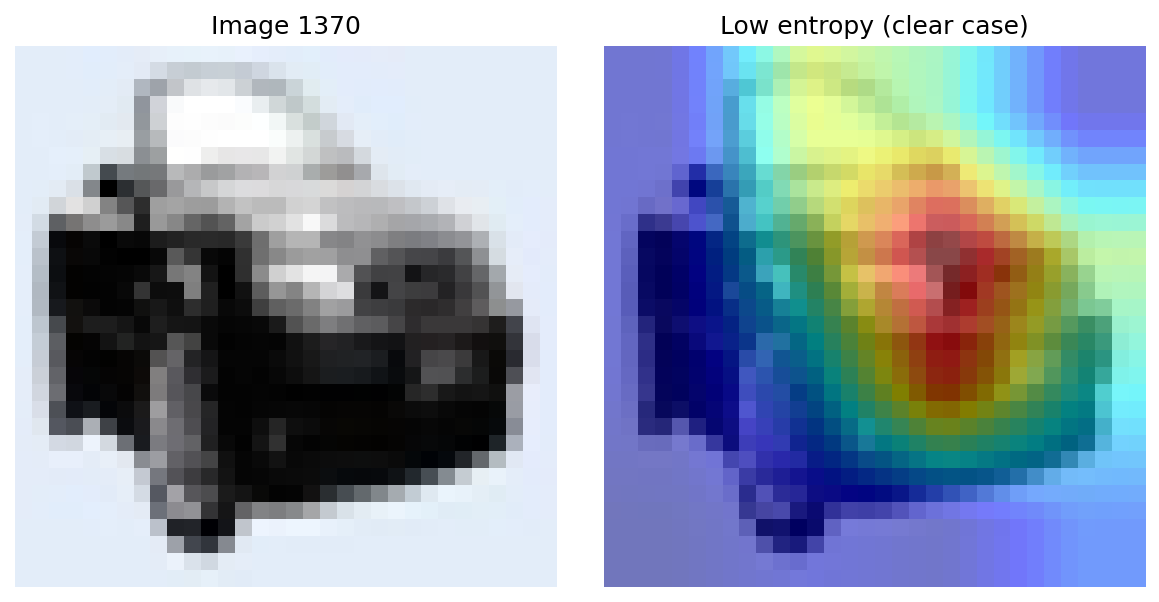
\includegraphics[width=0.3\textwidth]{figures/gradcam_low_entropy_00.png}
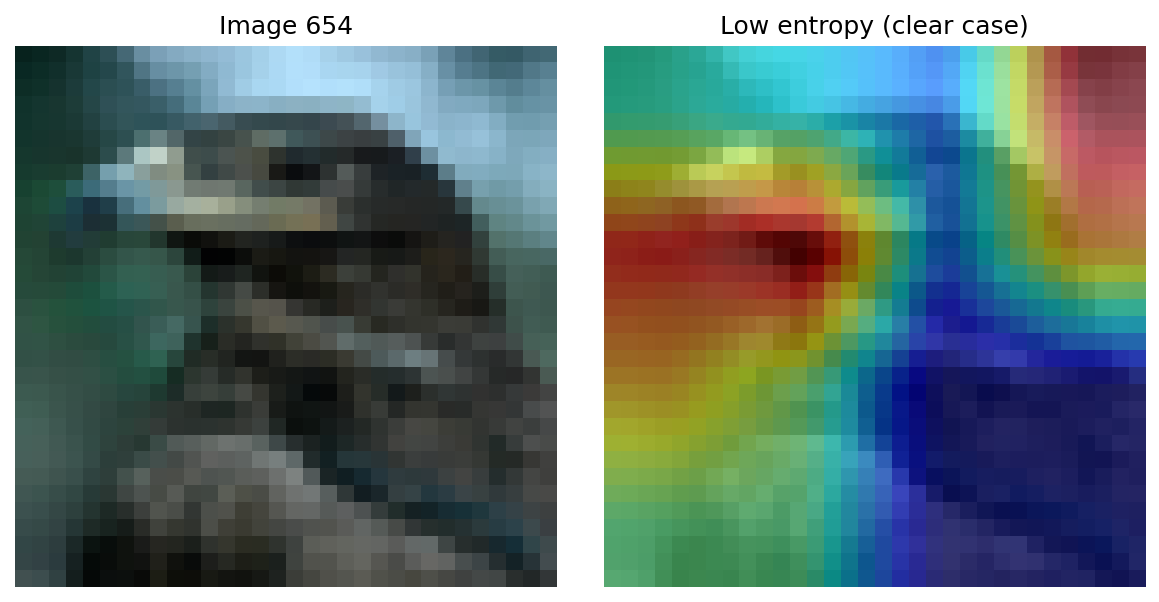
\includegraphics[width=0.3\textwidth]{figures/gradcam_low_entropy_01.png}
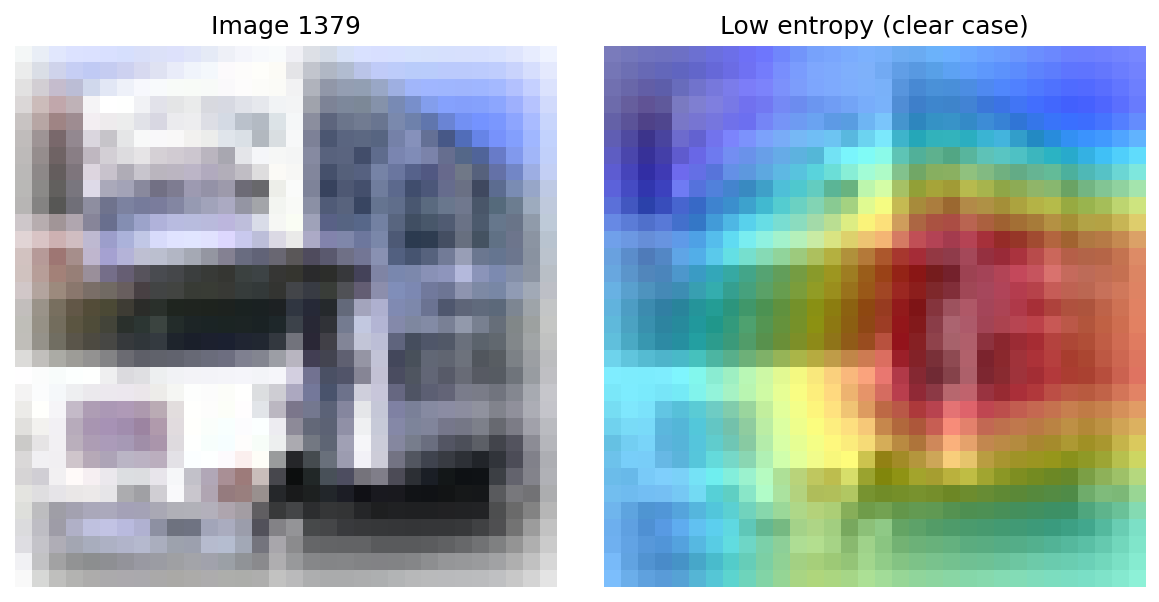
\includegraphics[width=0.3\textwidth]{figures/gradcam_low_entropy_02.png}

\vspace{6pt}

% Row 2
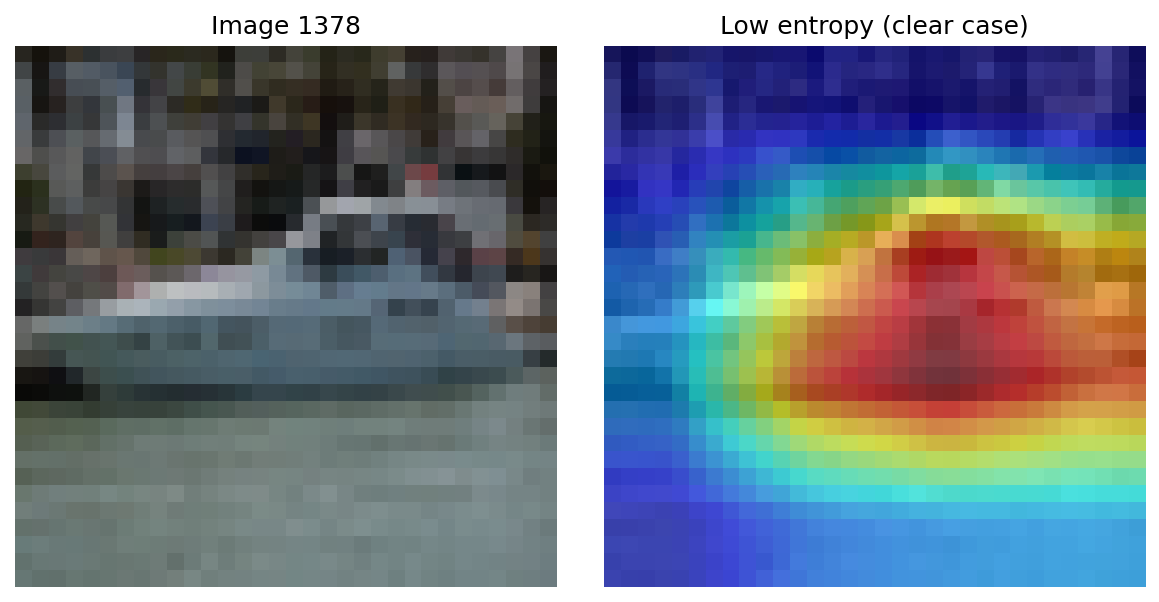
\includegraphics[width=0.3\textwidth]{figures/gradcam_low_entropy_03.png}
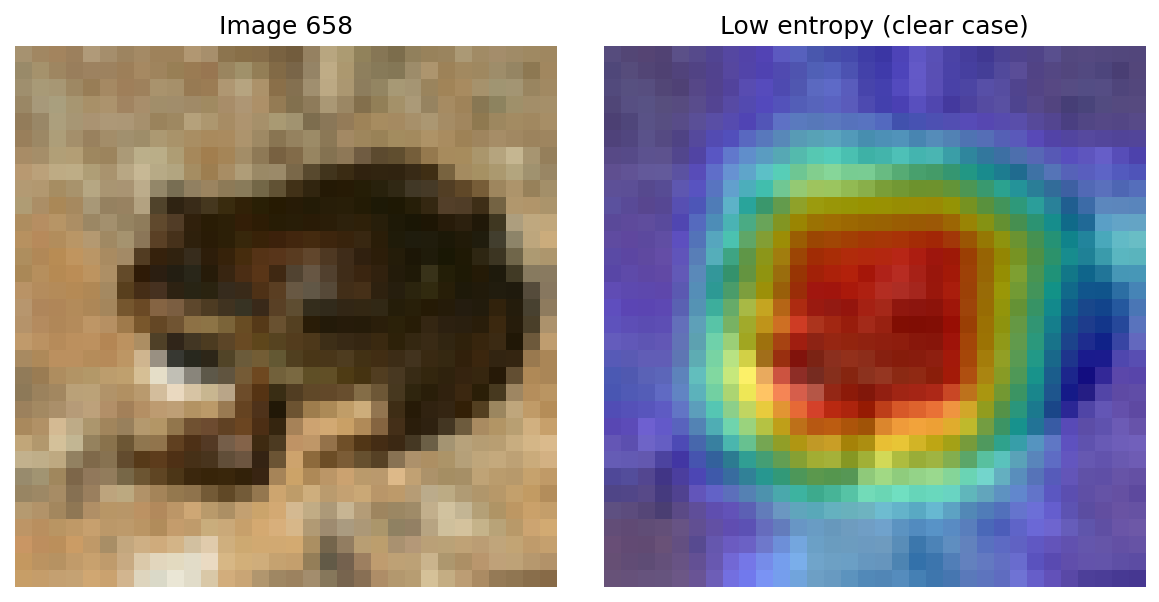
\includegraphics[width=0.3\textwidth]{figures/gradcam_low_entropy_04.png}

\caption{
Grad-CAM heatmaps for five low-entropy test images.
In all cases the model concentrates attention on the primary object region,
ignoring background.
This focused attention is consistent with the unambiguous nature of these
images: a single dominant feature drives a confident, peaked prediction.
}
\label{fig:gradcam_low}
\end{figure}

% ---------------- HIGH ENTROPY ----------------
\begin{figure}[H]
\centering

% Row 1
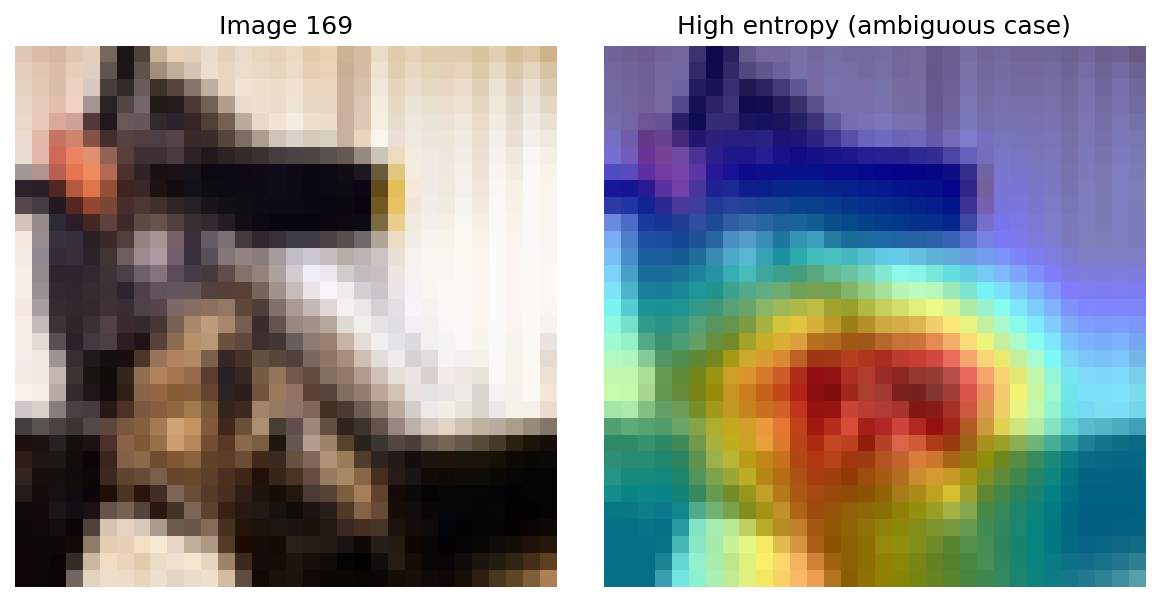
\includegraphics[width=0.3\textwidth]{figures/gradcam_high_entropy_00.png}
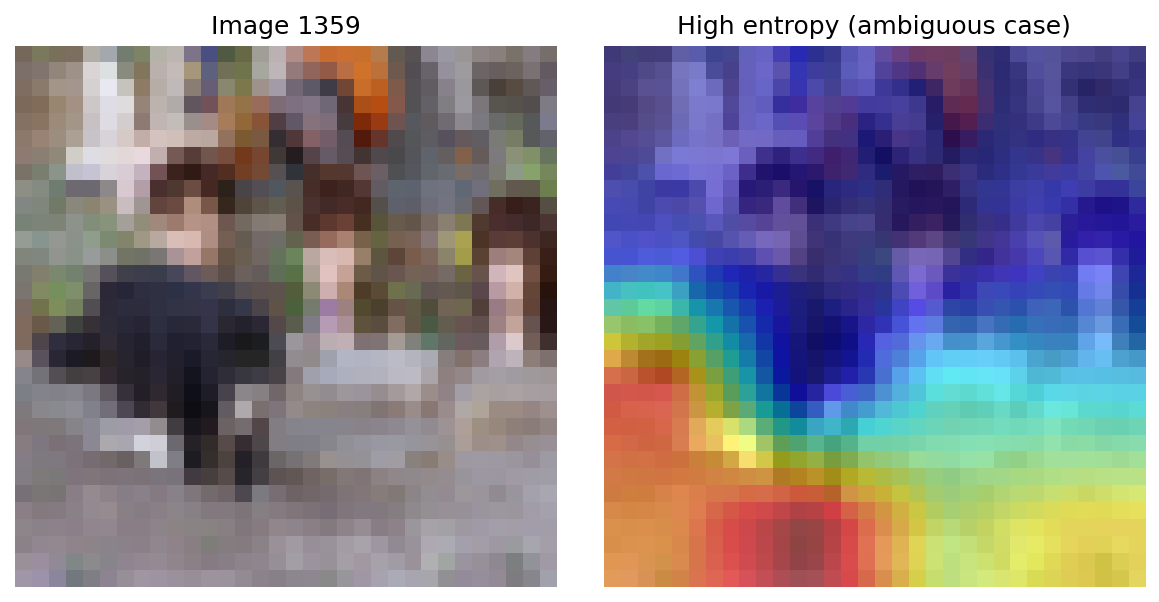
\includegraphics[width=0.3\textwidth]{figures/gradcam_high_entropy_01.png}
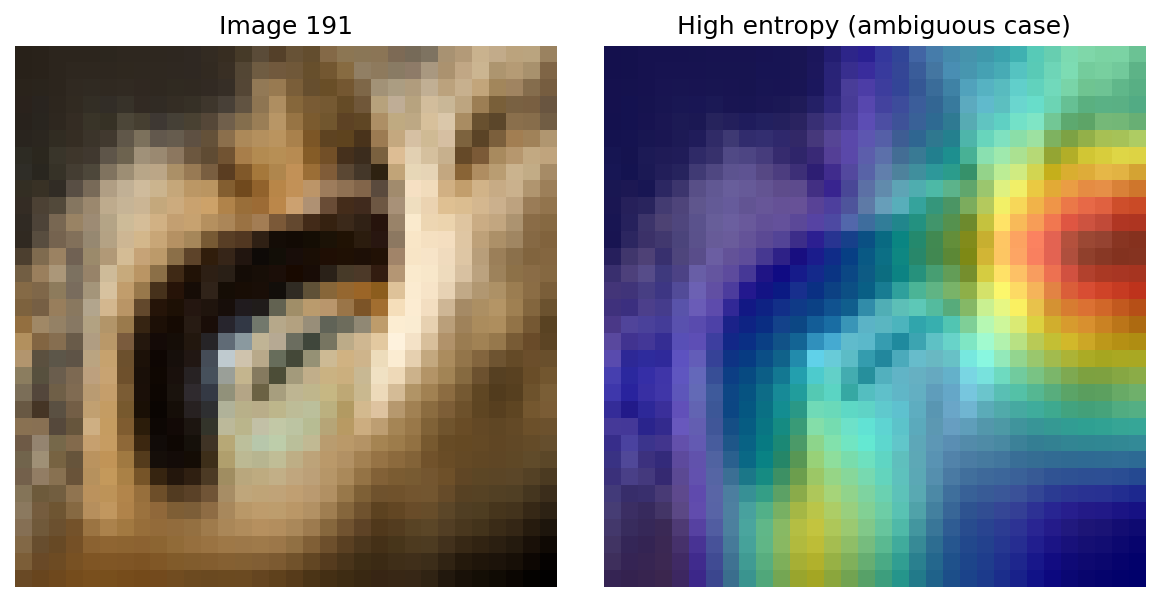
\includegraphics[width=0.3\textwidth]{figures/gradcam_high_entropy_02.png}

\vspace{6pt}

% Row 2
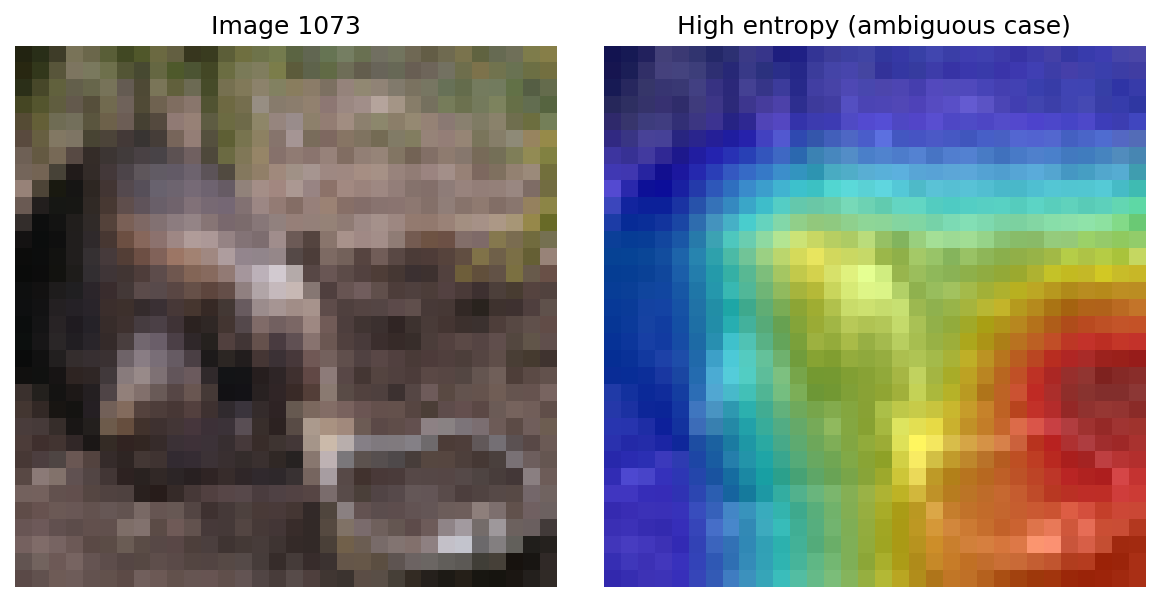
\includegraphics[width=0.3\textwidth]{figures/gradcam_high_entropy_03.png}
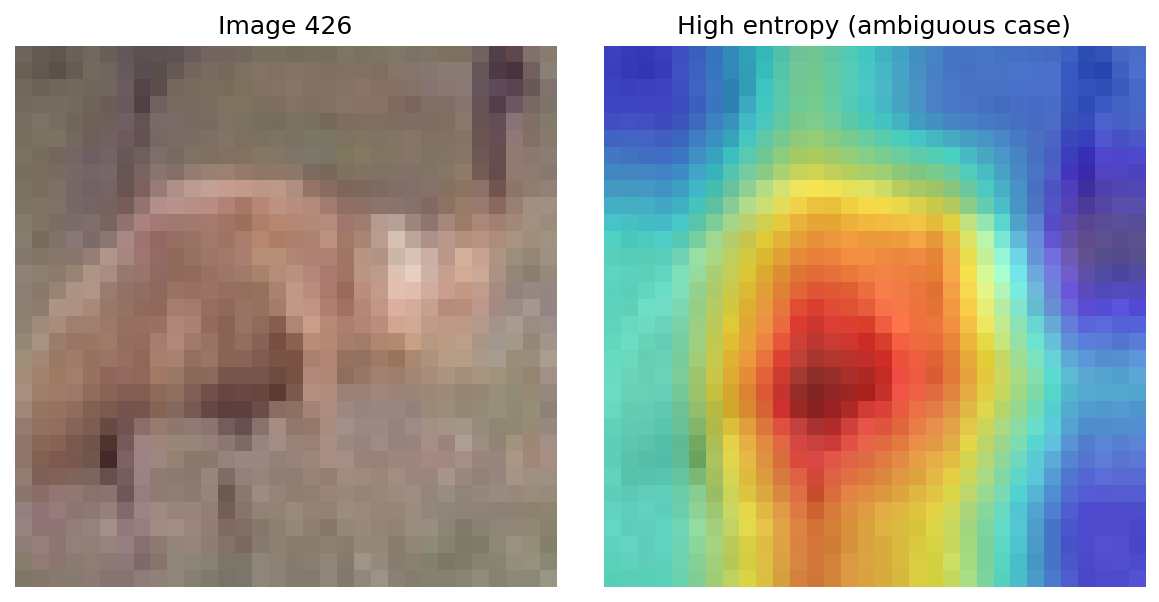
\includegraphics[width=0.3\textwidth]{figures/gradcam_high_entropy_04.png}

\caption{
Grad-CAM heatmaps for five high-entropy test images.
Attention is substantially more diffuse, often spread across background
regions or multiple candidate objects.
This pattern is consistent with genuine visual ambiguity: without a single
dominant feature, the model spreads probability mass, resulting in a
flatter, higher-entropy output distribution.
}
\label{fig:gradcam_high}
\end{figure}

\subsubsection{Failure Case Analysis}

Figure~\ref{fig:failures} shows the ten test images where the model's
predicted distribution most diverges from the true soft labels (highest
per-image KL divergence).

\begin{figure}[H]
\centering

% Row 1
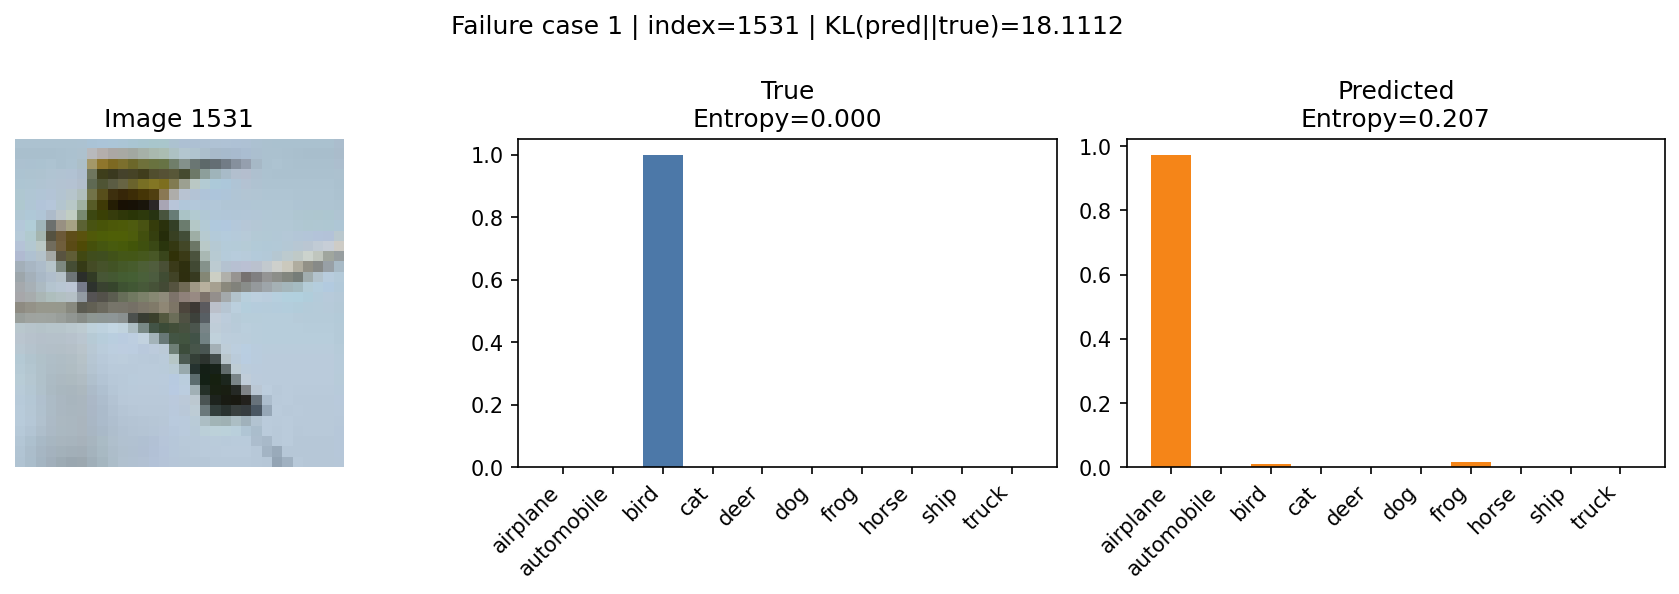
\includegraphics[width=0.48\textwidth]{figures/failure_case_00.png}
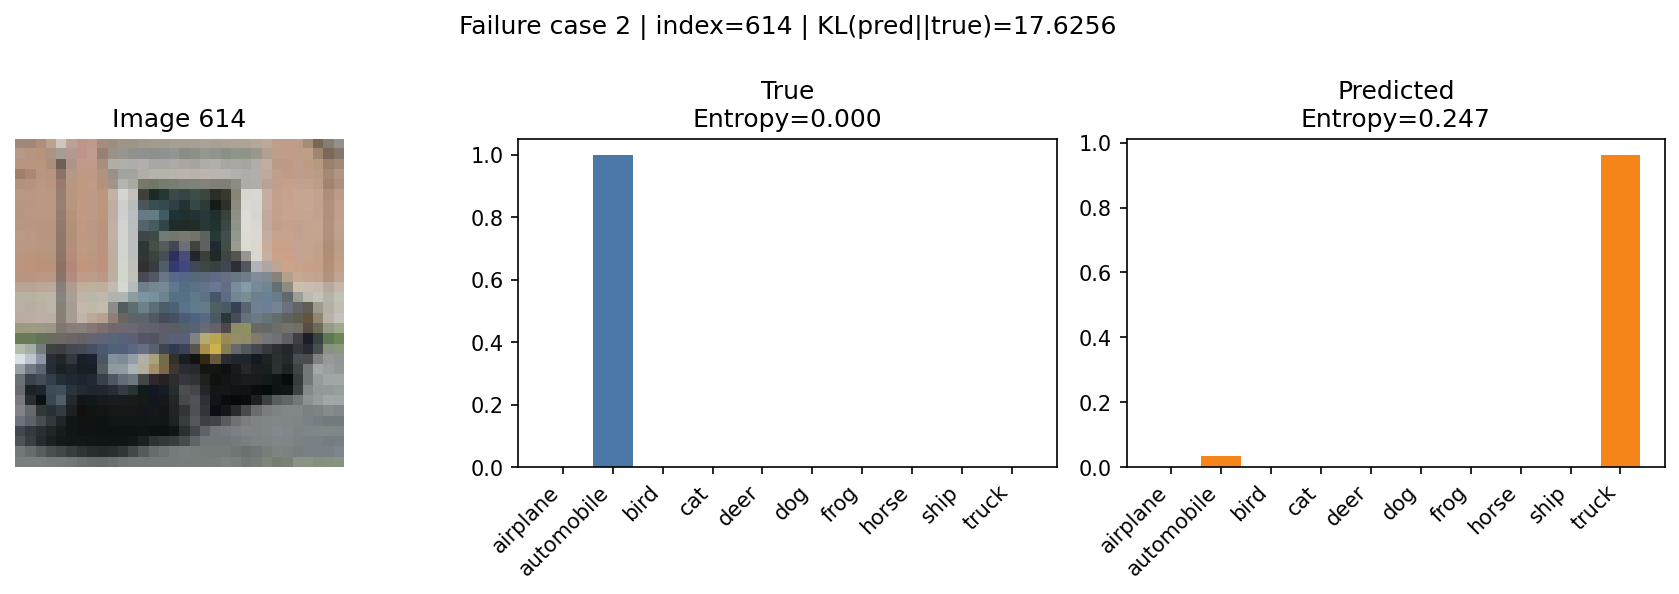
\includegraphics[width=0.48\textwidth]{figures/failure_case_01.png}

\vspace{6pt}

% Row 2
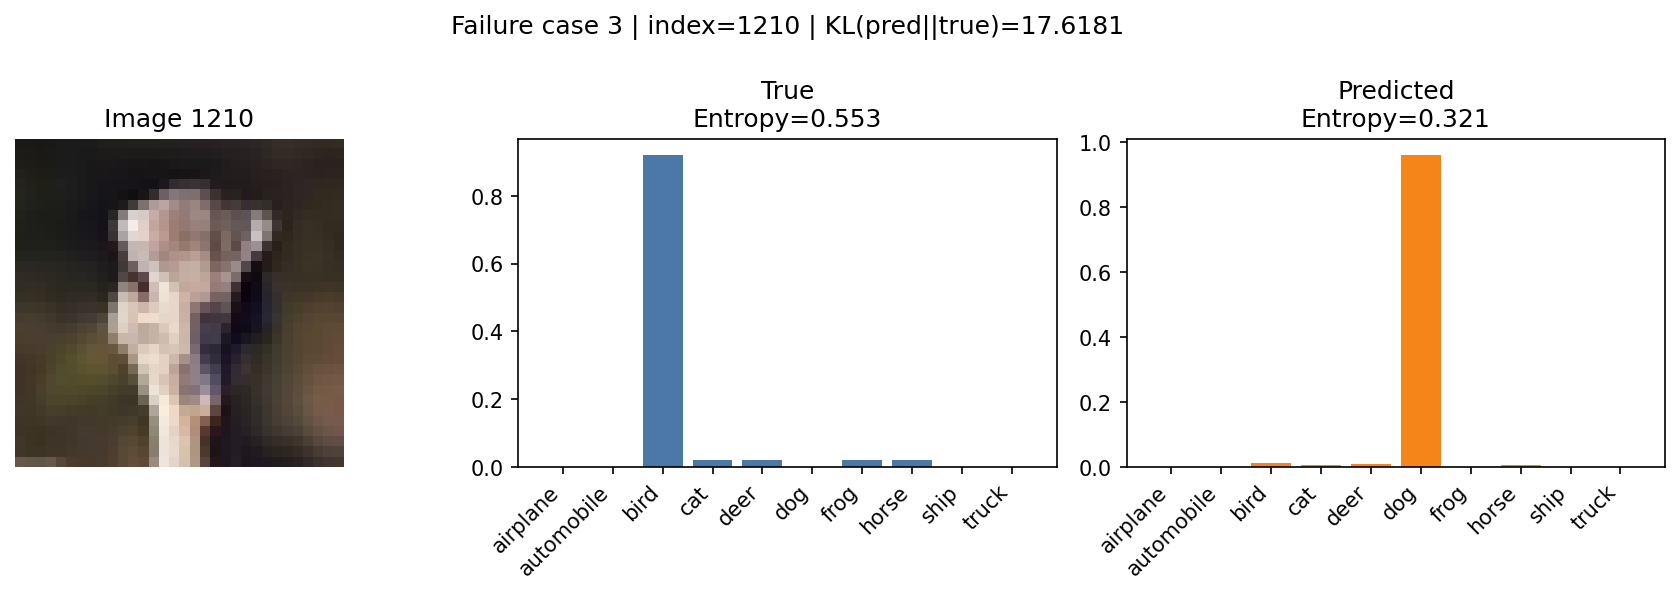
\includegraphics[width=0.48\textwidth]{figures/failure_case_02.png}
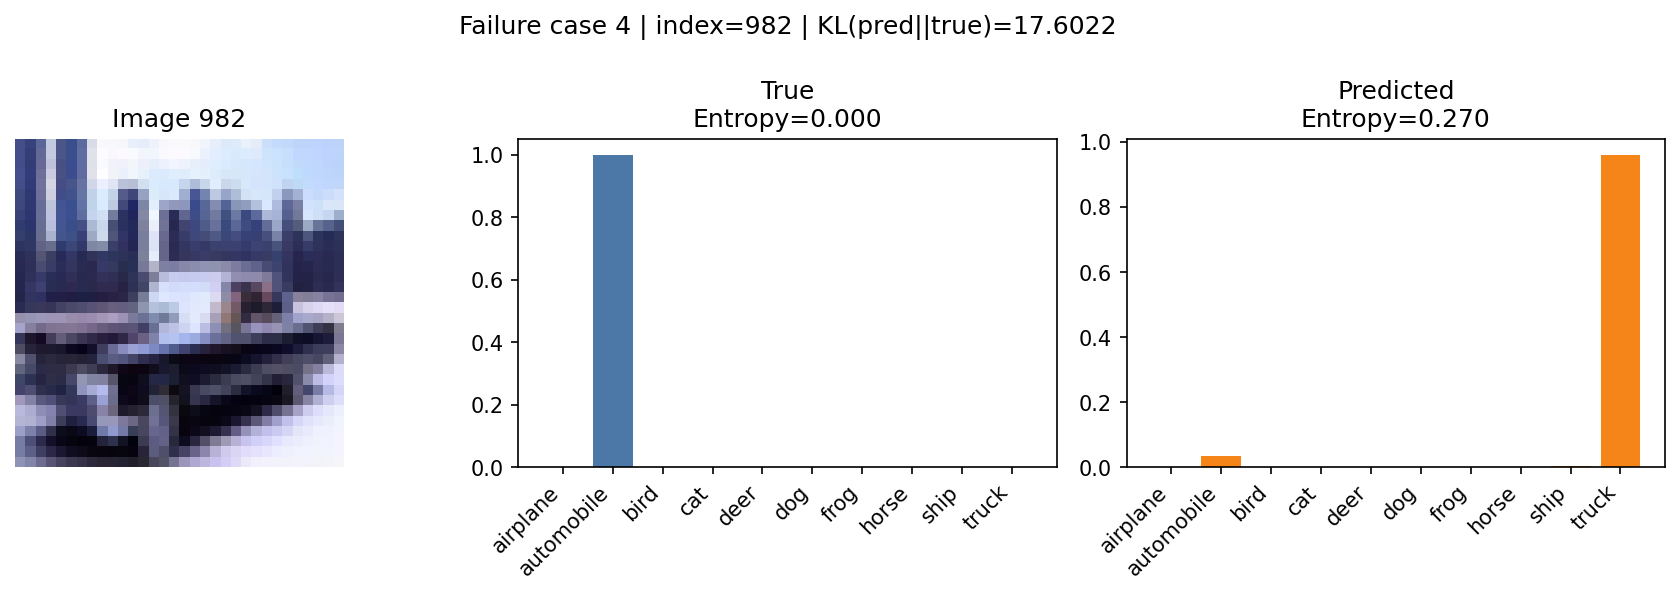
\includegraphics[width=0.48\textwidth]{figures/failure_case_03.png}

\vspace{6pt}

% Row 3
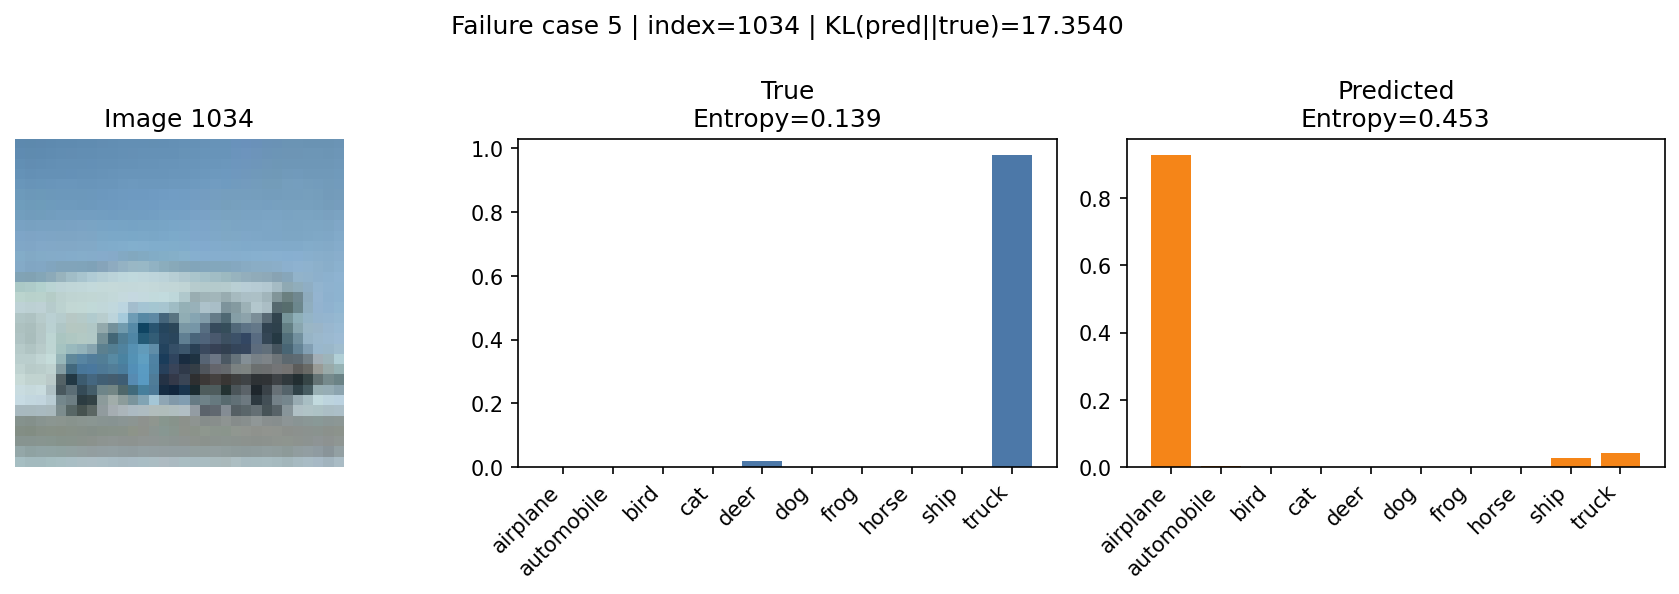
\includegraphics[width=0.48\textwidth]{figures/failure_case_04.png}
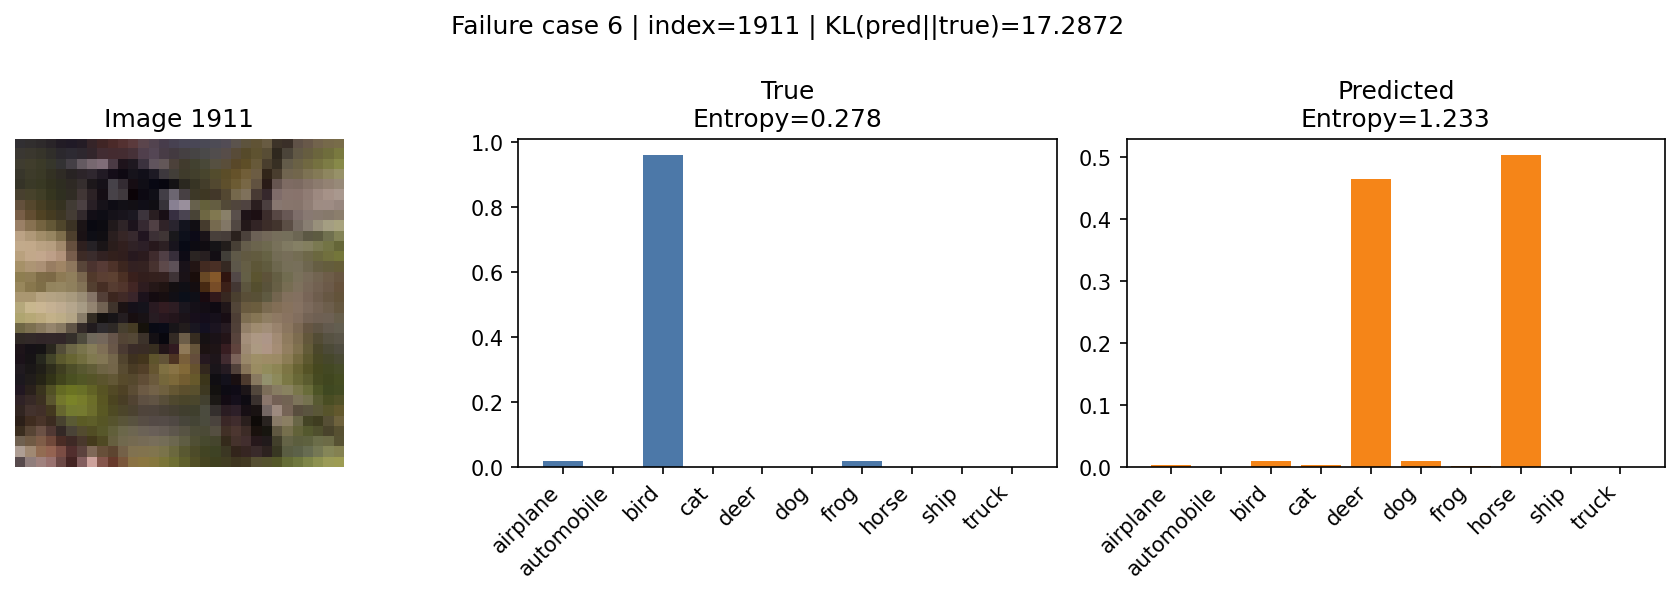
\includegraphics[width=0.48\textwidth]{figures/failure_case_05.png}

\vspace{6pt}

% Row 4
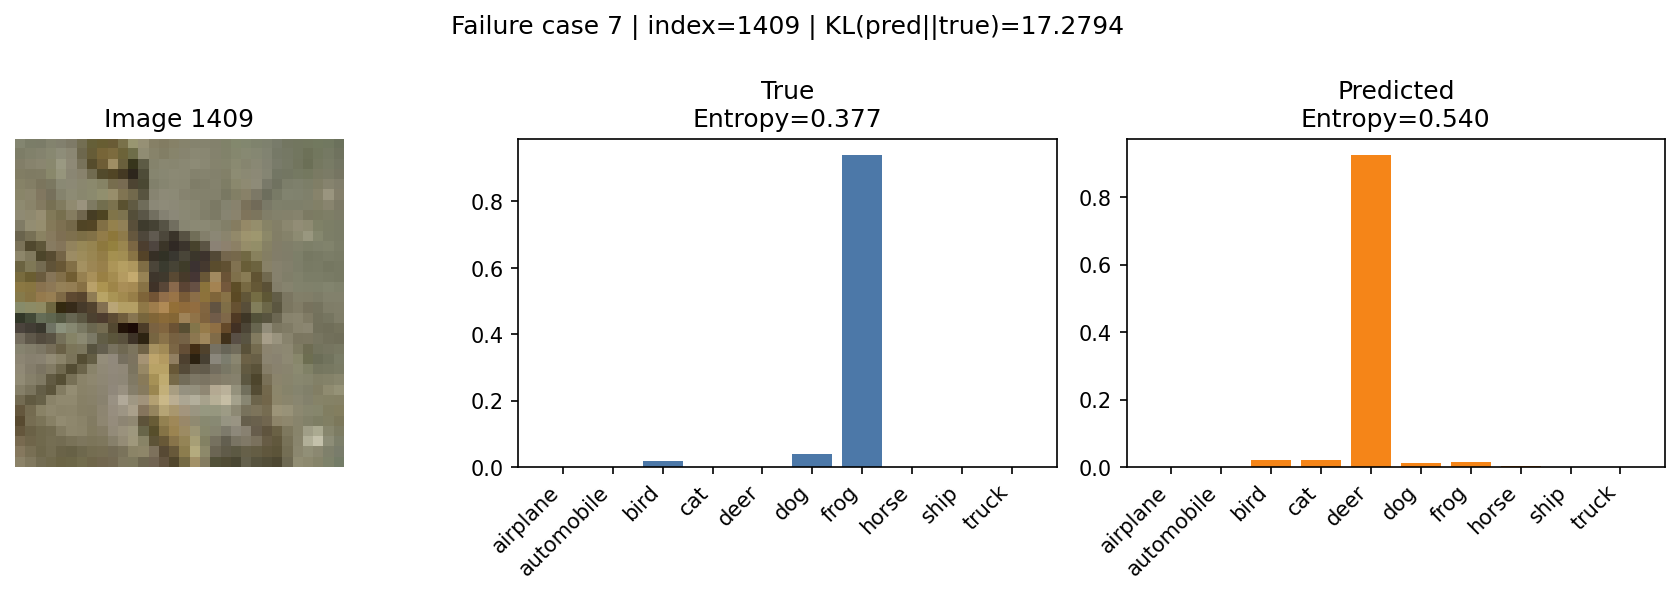
\includegraphics[width=0.48\textwidth]{figures/failure_case_06.png}
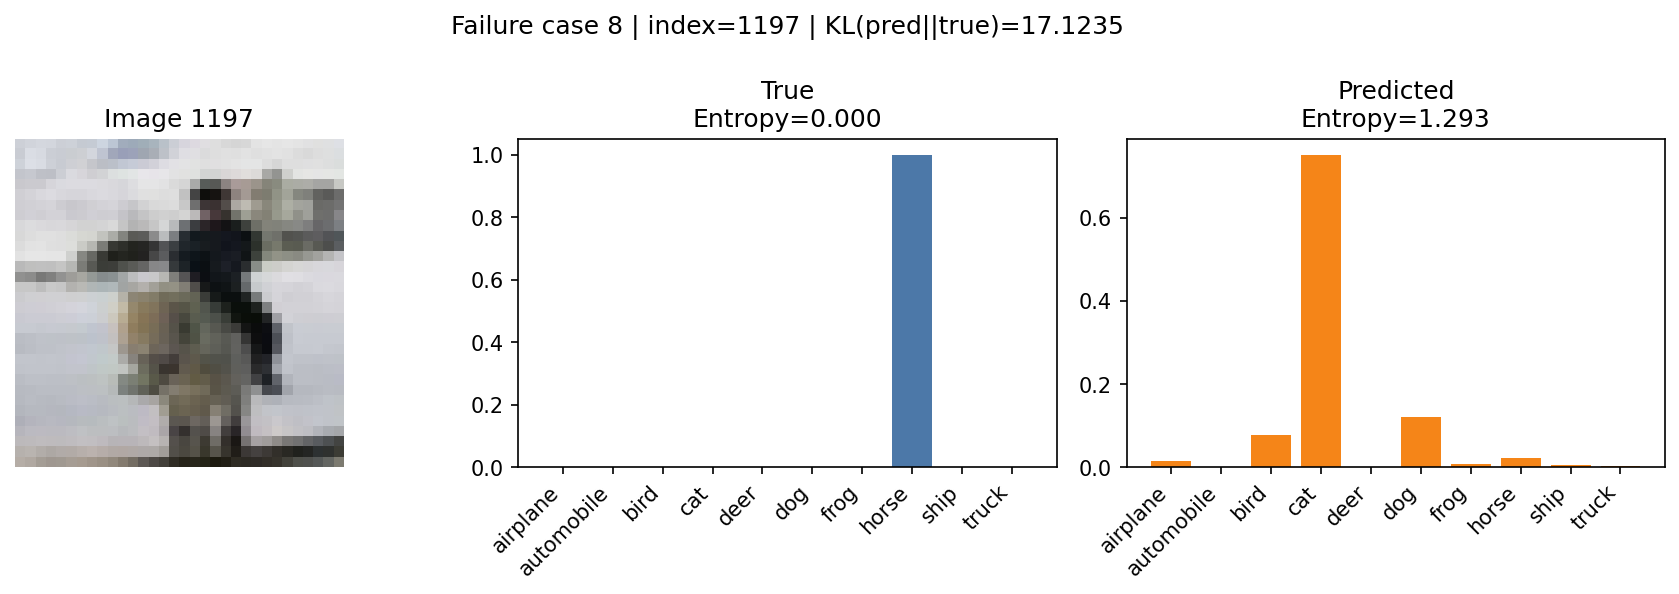
\includegraphics[width=0.48\textwidth]{figures/failure_case_07.png}

\vspace{6pt}

% Row 5
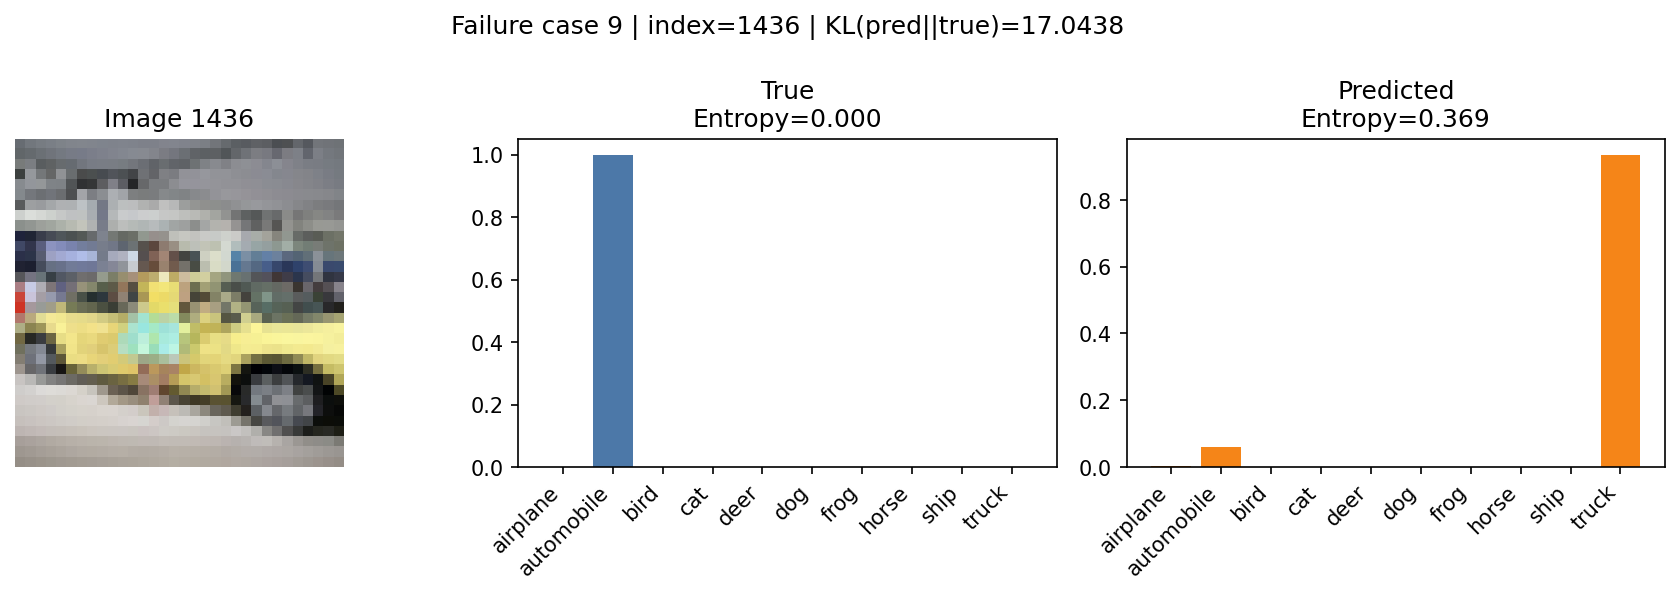
\includegraphics[width=0.48\textwidth]{figures/failure_case_08.png}
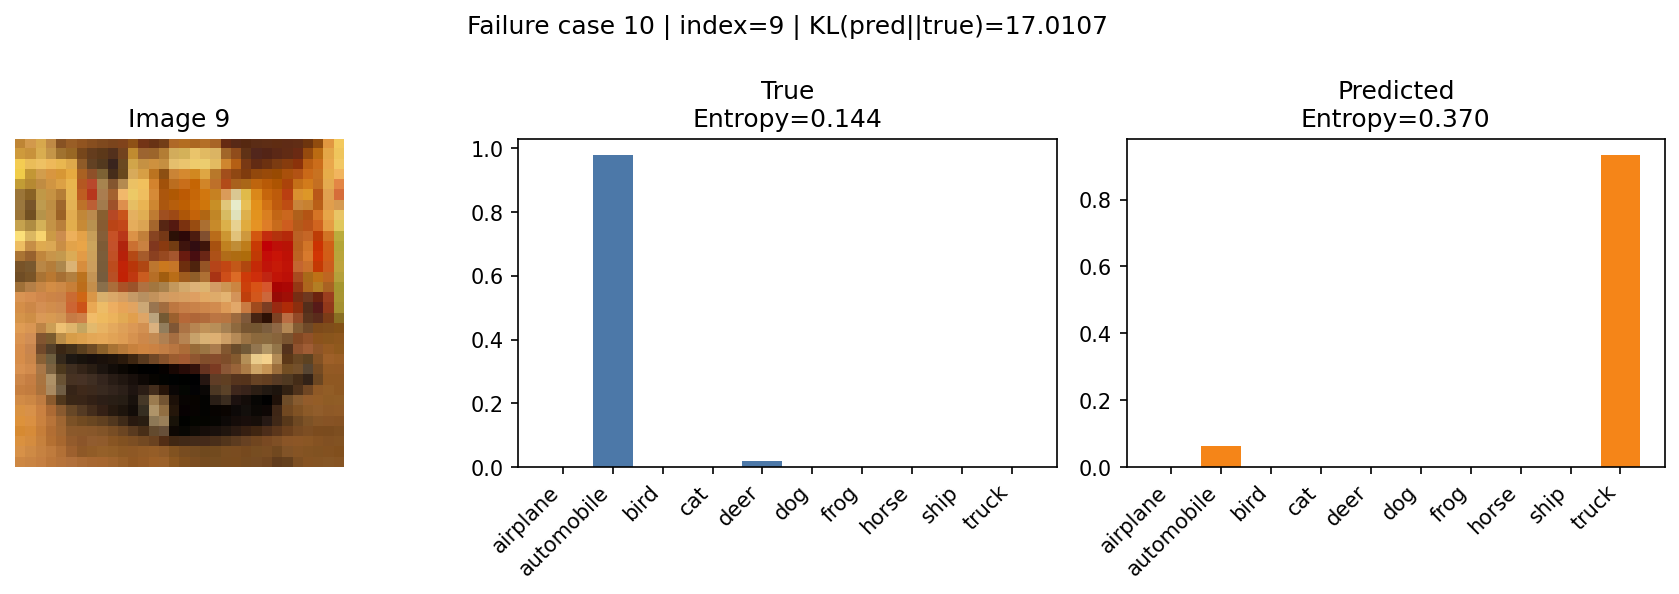
\includegraphics[width=0.48\textwidth]{figures/failure_case_09.png}

\caption{
Top-10 failure cases (highest per-image KL between prediction and
true soft label).
The dominant failure mode is \emph{entropy underestimation}: the model
predicts a sharply peaked distribution on images where annotators were
genuinely divided.
A secondary mode is \emph{wrong-mode prediction}: probability is
concentrated on a plausible-but-incorrect class, even when the true class
receives the largest human vote share.
}
\label{fig:failures}
\end{figure}
\subsubsection{Manual Disagreement Source Analysis}

We manually inspected 30 of the highest-entropy test images and categorised
each by its source of annotator disagreement.

\begin{table}[H]
\centering
\caption{Manual categorisation of 30 highest-entropy CIFAR-10H test images.}
\label{tab:manual}
\begin{tabular}{lrr}
\toprule
\textbf{Category} & \textbf{Count} & \textbf{Percentage} \\
\midrule
Ambiguous identity  & 11 & 36.7\% \\
Poor image quality  &  9 & 30.0\% \\
Boundary case       &  6 & 20.0\% \\
Multi-object scene  &  3 & 10.0\% \\
Ambiguous case      &  1 &  3.3\% \\
\midrule
Total               & 30 & 100\% \\
\bottomrule
\end{tabular}
\end{table}

\begin{figure}[H]
  \centering
  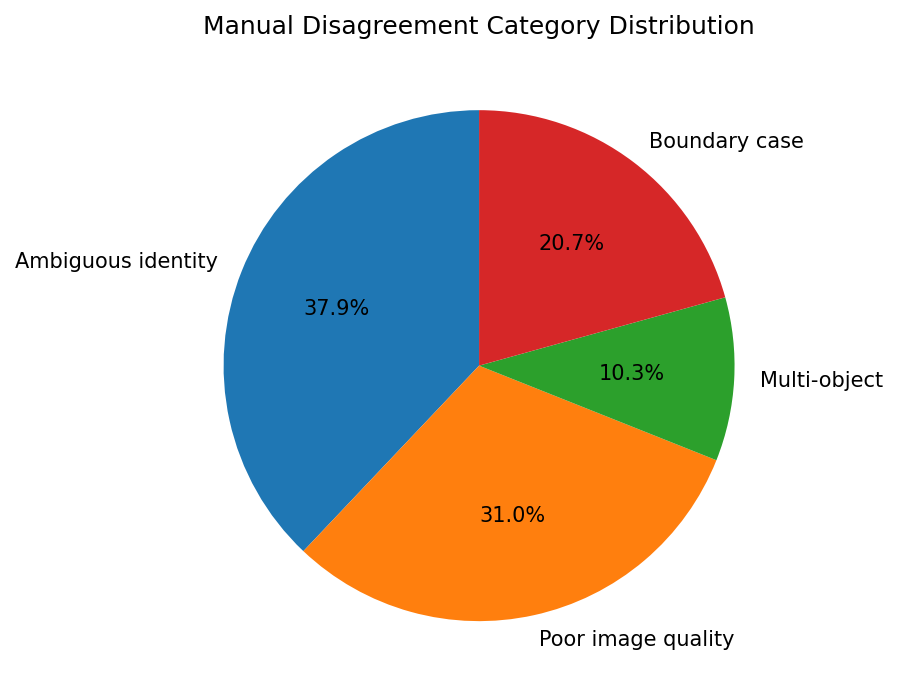
\includegraphics[width=0.50\textwidth]{figures/manual_disagreement_pie_chart.png}
  \caption{%
    Distribution of disagreement sources across the 30 highest-entropy test
    images.
    Ambiguous identity (36.7\%) and poor image quality (30.0\%) together
    account for two thirds of cases, identifying these as the primary
    drivers of human annotator uncertainty in CIFAR-10H.
  }
  \label{fig:manual_pie}
\end{figure}

The dominant cause of annotator disagreement is \emph{ambiguous identity}
(36.7\%): images where the depicted object genuinely resembles two or more
classes (e.g.\ a deer-like silhouette that could be mistaken for a horse).
\emph{Poor image quality} (30.0\%) is the second most frequent cause,
including blurry, dark, or low-contrast images where the object is difficult
to identify regardless of its true class.
\emph{Boundary cases} (20.0\%) involve objects at the semantic boundary
between adjacent categories.
\emph{Multi-object scenes} (10.0\%) contain more than one CIFAR-10 class,
making a single annotation genuinely ambiguous.

% ═══════════════════════════════════════════════════════════════════════════════
\section{Discussion}

\subsection{What Worked}

\paragraph{Entropy calibration improves disagreement prediction.}
The custom entropy-calibrated KL loss consistently outperforms both KL and JSD
on entropy-prediction metrics (Pearson $r$, Spearman $\rho$, all
Precision@$K$).
The explicit entropy penalty provides a gradient that supervises the
\emph{degree} of annotator disagreement, not just its direction — the most
practically useful property for downstream applications such as active
learning and data auditing.

\paragraph{CIFAR-10 pretraining is essential on small data.}
With only 6,000 training examples the choice of initialisation has a
pronounced effect.
CIFAR-10 pretrained features already encode the relevant visual distinctions
between CIFAR classes, allowing the model to specialise quickly on soft-label
regression.

\paragraph{Corruption robustness confirms calibrated uncertainty.}
Predicted entropy increases monotonically with corruption severity across all
tested types, demonstrating that the model correctly transfers its learned
notion of visual ambiguity to degraded inputs — a sign of well-calibrated
uncertainty.

\subsection{What Did Not Work and Why}

\paragraph{JSD underperforms relative to KL.}
Despite its theoretical stability advantages, JSD produces the worst results
on most metrics.
We attribute this to its bounded gradient magnitude: near the optimum, JSD
gradients are small and nearly uniform, making it difficult to distinguish
``almost correct'' from ``clearly wrong'' predictions on this small dataset.

\paragraph{All models systematically underestimate high entropy.}
All three scatter plots (Figure~\ref{fig:scatter_all}) show a systematic
compression: predicted entropy rarely exceeds ${\sim}1.5$ bits even for images
with true entropy up to $3$ bits.
This is a direct consequence of entropy class imbalance in the training set —
over 4,400 of 6,000 training images have near-zero entropy, so the model is
strongly penalised for high-entropy predictions and learns a conservative bias.

\paragraph{Temperature scaling is too rigid.}
A single global temperature cannot account for per-image variation in
uncertainty; it can only uniformly sharpen or spread the output distribution.
This explains why it performs similarly to the linear head on distribution
metrics but worse on entropy correlation.

\subsection{Limitations}

\begin{itemize}[noitemsep]
  \item The 6,000-image training set is small, particularly in the high-entropy
        regime; augmentation strategies that preserve visual ambiguity may help.
  \item Soft labels depend on the specific annotator pool, interface design,
        and task framing of the CIFAR-10H collection.
  \item The entropy calibration hyperparameter $\alpha = 0.5$ was not
        exhaustively tuned; a search over $\alpha$ may yield further
        improvements.
  \item EMD as a training loss was not explored due to non-differentiability
        via scipy; a differentiable implementation using the Python Optimal
        Transport (\texttt{pot}) library is a natural extension.
\end{itemize}

% ═══════════════════════════════════════════════════════════════════════════════
\section{Conclusion}

We have presented a systematic study of soft-label regression for predicting
human annotator disagreement on CIFAR-10H.
Our adapted ResNet-18 with an entropy-calibrated KL loss achieves test JSD of
0.0567 and Pearson $r = 0.421$, outperforming both standard KL and JSD on
five of eight metrics.

Ablation studies confirm that CIFAR-10 pretraining and a two-layer MLP head
provide the strongest foundation, while the two-stage training strategy
(hard-label pretraining then soft-label fine-tuning) outperforms direct
soft-label training alone.
Robustness checks demonstrate appropriate uncertainty escalation under OOD
corruptions.
Grad-CAM analysis reveals a clear qualitative difference in attention patterns
between low- and high-entropy images.
Manual inspection of the highest-entropy cases identifies ambiguous object
identity and poor image quality as the primary drivers of human annotator
disagreement.

Future work could explore richer uncertainty models (e.g.\ Dirichlet priors,
evidential deep learning), differentiable EMD training, and extension to
higher-resolution datasets with structured soft-label collection.

% ═══════════════════════════════════════════════════════════════════════════════
\printbibliography

\newpage
\appendix

\section{Hyperparameter Configuration}
\label{app:config}

\begin{table}[H]
\centering
\caption{Complete hyperparameter configuration (\texttt{config.py}).}
\label{tab:config}
\begin{tabular}{ll}
\toprule
\textbf{Parameter} & \textbf{Value} \\
\midrule
\texttt{SEED}                      & 42 \\
\texttt{BATCH\_SIZE}               & 64 \\
\texttt{LR}                        & $10^{-3}$ \\
\texttt{WEIGHT\_DECAY}             & $10^{-4}$ \\
\texttt{EPOCHS}                    & 150 \\
\texttt{EARLY\_STOPPING\_PATIENCE} & 15 \\
\texttt{CIFAR10H\_TRAIN\_SIZE}     & 6{,}000 \\
\texttt{CIFAR10H\_VAL\_SIZE}       & 2{,}000 \\
\texttt{CIFAR10H\_TEST\_SIZE}      & 2{,}000 \\
\texttt{ENTROPY\_ALPHA}            & 0.5 (custom loss only) \\
\bottomrule
\end{tabular}
\end{table}

\section{Additional Figures}
\label{app:figs}

\begin{figure}[H]
  \centering
  
\includegraphics[width=0.70\textwidth]{figures/classwise_jsd.png}
  \caption{Class-wise JSD bar chart for all three loss functions across all
  ten CIFAR-10 classes.}
\end{figure}

\end{document}
